% das Dokumentenformat
\documentclass[a4paper, 12pt, oneside]{article}

\usepackage[T1]{fontenc}
\usepackage[utf8]{inputenc}
\usepackage{lmodern}

%% IMAGE PACKAGE
\usepackage{graphicx}

%% PACKAGE FOR THE BACKGROUNDPIC
\usepackage{eso-pic}

%% PACKAGE FOR THE HEADERS AND FOOTERS
\usepackage{fancyhdr}

%% PACKAGE TO INCLUDE A PDF FILE
\usepackage{pdfpages}

%% TABLES
\usepackage{booktabs}
\usepackage{multirow}
\usepackage{array}
\usepackage{float}
\usepackage{longtable}
\usepackage{tabularx}

%% MATH
\usepackage{amsmath,amssymb}

%% LISTS
\usepackage{enumitem}

%% LINKS
\usepackage[hyphens]{url}
\usepackage{xcolor}
\usepackage[colorlinks=true,linkcolor=blue!60!black,citecolor=blue!60!black,urlcolor=blue!60!black]{hyperref}

%% TYPOGRAPHY
\usepackage{microtype}
\setlength{\emergencystretch}{3em}

%% CITATIONS
\usepackage[numbers,sort&compress]{natbib}

%% CAPTIONS
\usepackage{caption}

% Keep the electronic PDF centered instead of using mirrored print-binding margins.
\setlength{\oddsidemargin}{\dimexpr(\paperwidth-\textwidth)/2-1in\relax}
\setlength{\evensidemargin}{\oddsidemargin}

\newcommand\BackgroundPic{%
\put(0,0){%
\parbox[b][\paperheight]{\paperwidth}{%
\vfill
\centering

\includegraphics[width=\paperwidth,height=\paperheight,keepaspectratio]{background.pdf}%
\vfill
}}}
\fancyhf{}% Clear all headers/footers
\renewcommand{\headrulewidth}{0pt}% No header rule
\renewcommand{\footrulewidth}{0pt}% No footer rule
\fancyfoot[L]{\hspace*{-16mm}
\includegraphics[scale=0.3]{logoDepartment.pdf}}

\begin{document}

\AddToShipoutPicture*{\BackgroundPic}
\thispagestyle{fancy}

{\vspace{2cm}~}
{\vspace{2cm}}

{\noindent\large Bachelor Thesis}

\vspace{1cm}

{\noindent\huge\bfseries
Comparing Machine Learning\\
Approaches for Trade Intent\\
Classification from Noisy\\
Livestream Transcripts\par}

\bigskip

{\noindent\LARGE Andreas Oberd\"orfer}

\bigskip
{\noindent\small Date of Birth: 24.12.2002}\newline
{\noindent\small Student ID: h12217505}

\bigskip
{\vspace{2cm}}
{\noindent\large {\bf Subject Area:} Information Business}

\bigskip
{\noindent\large {\bf Studienkennzahl:} J 033 561}

\bigskip

{\noindent\large {\bf Supervisor:} Johann Mitl\"ohner}

\bigskip

{\noindent\large {\bf Date of Submission:} 26.06.2026}

\bigskip\bigskip\bigskip\bigskip\bigskip\bigskip

{\em\noindent Department of Information Systems \& Operations Management, Vienna University of
Economics and Business, Welthandelsplatz 1, 1020 Vienna, Austria
}


\pagebreak
\tableofcontents
\pagebreak
\listoffigures
\pagebreak
\listoftables
\pagebreak


\begin{abstract}

Day traders often stream live on platforms like YouTube, talking through their trades as they happen. Buried in that constant talk are the moments that matter: when they buy, sell, or move a stop. Pulling out these signals automatically means first turning the speech into text with automatic speech recognition (ASR), then sorting each line into a trading action, a task made hard by recognition errors, casual language, and far more chatter than actual trade calls.

The thesis frames this as a seven-class problem, assigning each transcript line one trading action, and compares five machine learning methods on it. Three are classical, reading simple word-count (TF-IDF) features: logistic regression, a support vector machine, and a compact neural network. The other two are recent transformer models, DistilBERT and ModernBERT, used in a lightweight way, with their inner layers frozen so that only a small classifier on top is trained. All five meet the same labelled benchmark under an identical procedure, so the comparison is fair.

The simple word-count methods come out ahead. Logistic regression is strongest, with a macro-averaged F1 of 0,70 and an F1 of 0,89 for telling action lines from commentary. The reason is that a handful of trading keywords carries most of the signal, which TF-IDF captures directly, while the frozen transformers, never tuned for the task, read this narrow vocabulary no better despite their far greater size. Keyword-driven actions such as trimming, exiting, or moving a stop are easy to flag; entries are hard, because traders phrase them in countless ways. The lesson is that on a small, specialised, repetitive dataset, word-count features stay highly competitive, and a transformer's added complexity pays off only when the model is actually trained on the task. A closing test on five complete held-out sessions then exposes what the benchmark hides: set loose on a real stream, even the best model raises far more false alarms than real signals, so on its own it is unusable. The production system therefore puts the model in a supporting role behind strict hand-written rules; replayed over those sessions it fires about six times an hour instead of 225, with roughly one fire in six hitting a real action, yet it still misses most labelled actions, making it a workable alerting aid rather than a fully automatic trade copier.

\medskip
\noindent\textbf{Keywords:} text classification, trade intent detection, TF-IDF, support vector machine, logistic regression, transformer models, DistilBERT, ModernBERT, automatic speech recognition, livestream transcription
\end{abstract}

\pagebreak

\section{Introduction}
\label{sec:introduction}

\subsection{Motivation}
\label{sec:motivation}

The growth of live-streaming has created a new kind of real-time financial commentary. On YouTube and Twitch, day traders share their screens and talk through their trades as they happen, calling out when they buy, when they sell, when they adjust a position, and when they move a stop-loss, all in natural spoken language. For a viewer who wants to follow or copy these trades, the problem is easy to state: the useful signals are buried in hours of talking that also include market analysis, replies to chat, personal stories, and long silences. Spotting the exact moment a trader commits to a trade takes constant attention, and the moment a viewer looks away, a signal can slip by. In day trading, timing often decides whether a trade ends as a win or a loss, so a signal noticed late is worth little.

These streams are popular. During market hours, well-known day-trading channels draw thousands of viewers at once, many of them following a single instrument such as the E-mini Nasdaq futures (NQ). But unlike written trade alerts posted on social media, what a streamer says is short-lived and unstructured. The line between just thinking out loud (``I'm watching this level'') and actually committing (``I'm long here'') can be subtle and depends on the context.

This is what motivates an automated system that can do three things: (1)~turn the live audio into text as it happens, (2)~decide which lines of that text actually contain a trade signal, and (3)~sort each signal into a concrete action, such as ``enter long,'' ``trim position,'' or ``move stop.'' The first step, turning speech into text, has been transformed by recent large models such as Whisper~\cite{radford2023whisper}, which turn speech into text with an accuracy close to a human transcriber. The second and third steps are a text classification problem: given a short line of transcript and the current trading context, choose one label from a fixed list.

At its heart, this is text classification, one of the most studied problems in natural language processing (NLP)~\cite{kowsari2019text}. Classical methods that count words and feed them to a simple linear model have long done well on tasks like sorting positive reviews from negative ones, or spam from real email~\cite{joachims1998text}. More recently, large pretrained models called transformers, such as BERT~\cite{devlin2019bert}, have set new records on many NLP benchmarks by learning rich, context-aware representations of words from huge amounts of text. But bigger is not always better. On small, specialised datasets this advantage can vanish, because a model trained on general text may simply miss the niche vocabulary that actually matters here~\cite{kowsari2019text}. That raises the central question: is the extra complexity of a transformer worth it for a task like this one?

Several problems show up at once in this domain. First, the language is casual and full of trader slang (``peel some off,'' ``add to the runner,'' ``move to breakeven''). Second, the speech-to-text step adds its own mistakes: specialist terms and sound-alike words are often misheard, in ways that change how the text looks to a classifier; Section~\ref{sec:asr} shows concrete examples. Third, the classes are very unbalanced, because most of what a trader says is commentary, not an actual trade call. Fourth, the same action can be said in many ways: a trader going long might say ``I'm long here,'' ``let's try it,'' ``small size,'' or just ``here we go.'' Finally, the dataset built for this work is small by modern NLP standards, with fewer than 1.500 labelled examples. Taken together, these traits make the task a well-suited test case for comparing classical and modern model families under realistic conditions.

\subsection{Research Question}
\label{sec:research_question}

The central question addressed in this work is:

\begin{quote}
\emph{Which approach gives the most accurate trade-intent classification on noisy livestream transcripts: classical TF-IDF methods or pretrained transformer models? And on a small, specialised dataset, does the extra complexity of a transformer actually buy any measurable improvement over the simpler methods?}
\end{quote}

To answer this, five models, three classical and two transformer-based, are compared under identical conditions: trained and tested on the same labelled data and scored with the same procedure, so that any difference in results comes from the model itself and not from the setup. Two follow-up questions are also examined: (1)~Which trading actions are easiest to detect automatically, which are hardest, and why? (2)~When a model gets a line wrong, what kinds of mistakes does it tend to make, and how do those mistakes relate to the way traders speak?

\subsection{Scope}
\label{sec:scope}

The scope of this thesis is deliberately narrow. The classification task is studied on its own: each model receives a short, ready-made piece of text containing one transcript line plus its trading context, and returns a single predicted action. The speech-recognition step before it and the trade-execution step after it are described for context but are not tested or tuned here. Only English-language streams are used. All labelled data comes from recorded streams of a single YouTube streamer, FlowzoneTrader, who day-trades the E-mini Nasdaq futures (NQ), so the results may not carry over to other traders, instruments, or styles.

All transformer models are also used with their encoder frozen: the large pretrained part of the model that reads the text stays unchanged, and only a small classifier on top is trained on the labelled data. Fully retraining the transformers (called fine-tuning) is not explored here, because it would need a much larger dataset to work safely. The same applies to LoRA, a lighter-weight form of fine-tuning that adjusts only a few small add-on weights inside the model instead of all of them; it is discussed as future work (Section~\ref{sec:future_work}).

\subsection{Structure of This Work}
\label{sec:structure}

The remainder of this thesis is organized as follows. Section~\ref{sec:related_work} introduces the concepts this work builds on, from text classification with TF-IDF features to transformer models and automatic speech recognition, and reviews related research on NLP in financial markets. Section~\ref{sec:methodology} describes the experiment: the system around the classifier, the exact classification task and its labels, how the dataset was built, checked, and cleaned, the five models, and the evaluation procedure. Section~\ref{sec:results} presents the results, Section~\ref{sec:discussion} discusses what they mean and where their limits lie, and Section~\ref{sec:summary} summarizes the question, the procedure, and the findings.


% ═══════════════════════════════════════════════════════════════
% 2. RELATED WORK
% ═══════════════════════════════════════════════════════════════
\section{Related Work}
\label{sec:related_work}

This section reviews the methods and research areas that form the foundation of the present work. The discussion proceeds from general text classification concepts to the specific model families evaluated, then covers the speech recognition technology that generates the input data, and concludes with a survey of NLP applications in financial markets.

\subsection{Text Classification}
\label{sec:text_classification}

Text classification, the task of assigning predefined labels to natural-language documents, is a foundational NLP task spanning spam filtering, sentiment analysis, topic categorization, and intent detection~\cite{kowsari2019text}. Approaches differ mainly in how text is represented (engineered features versus learned representations) and in the complexity of the classifier (linear versus nonlinear).

Early opinion-mining work by Hu and Liu~\cite{hu2004mining} showed that sentiment could be extracted from unstructured reviews with relatively simple pattern-based and statistical methods, establishing that domain-specific lexical patterns are often highly predictive even without deep syntactic or semantic analysis; later surveys such as Percha's clinical-text-mining review~\cite{percha2021modern} trace the evolution from rule-based systems to neural methods while stressing that the choice should be guided by the data rather than the novelty of the method. A consistent finding is that the quality and representativeness of the training data often matter more than the algorithm~\cite{kowsari2019text}: small, noisy, or imbalanced datasets can nullify the advantages of sophisticated models, while careful curation and feature engineering can compensate for architectural simplicity. This foreshadows the central tension of the present work: whether the richer representations of pretrained transformers overcome the disadvantage of a small, noisy, domain-specific corpus, or whether the corpus characteristics dominate.

\subsection{Feature Extraction: TF-IDF}
\label{sec:tfidf}

Term Frequency--Inverse Document Frequency (TF-IDF) is a classical text representation scheme that assigns a numerical weight to each word in a document based on two factors: how frequently the term appears in the document (term frequency) and how rare it is across the entire corpus (inverse document frequency)~\cite{salton1988term, manning2008introduction}. Formally, for a term~$t$ in a document~$d$ within a corpus~$D$:

\begin{equation}
\text{TF-IDF}(t, d, D) = \text{tf}(t, d) \times \log\!\left(\frac{|D|}{|\{d' \in D : t \in d'\}|}\right)
\label{eq:tfidf}
\end{equation}

\noindent where $\text{tf}(t, d)$ denotes the frequency of term~$t$ in document~$d$, and the logarithmic factor downweights terms that appear in many documents. Sublinear scaling of the term frequency component ($1 + \log(\text{tf})$ instead of raw~$\text{tf}$) is commonly applied, so that a term occurring ten times counts only a little more than one occurring twice~\cite{manning2008introduction}.

Because the word \emph{feature} appears throughout this thesis, it is worth pinning down early. A feature is one measurable property of the input that a model can use for its decision. In TF-IDF, every distinct word seen in the training texts becomes one feature, and its value for a given document is the weighted count from Equation~\ref{eq:tfidf}. Pairs of neighbouring words are usually included as features as well: a single word is called a \emph{unigram}, a two-word sequence a \emph{bigram}. The line ``taking a partial here'' thus switches on the unigram features ``taking,'' ``partial,'' and ``here'' and the bigram features ``taking partial'' and ``partial here'' (very short words such as ``a'' are skipped). Each document becomes a long list of numbers, one per feature, almost all of them zero. Despite its simplicity, this representation has proven remarkably effective for text classification, particularly when combined with linear classifiers~\cite{joachims1998text}: it is interpretable (each feature is a human-readable word or phrase), cheap to compute, and it picks up domain-specific vocabulary directly from the training data, with no need for pretrained models or word lists from outside.

TF-IDF has one big weakness: it treats every word on its own. It ignores word order, and it ignores meaning, so two lines that mean the same thing but use different words share no features at all. For example, ``I'm long here'' and ``just bought a few'' both signal a buy, but because they have no words in common, TF-IDF sees them as completely unrelated. This is exactly the gap that word embeddings, covered in the next sections, are meant to close. That said, keying on exact words turns out to suit trading talk very well, because traders tend to repeat the same handful of action words (``trim,'' ``stop,'' ``long''); the feature-importance analysis in Section~\ref{sec:feature_importance} shows this directly.

\subsection{Classical Classification Algorithms}
\label{sec:classical_classifiers}

Three classical classification algorithms are evaluated in this work, all applied to TF-IDF feature vectors.

\textbf{Logistic Regression} is a linear model that predicts class probabilities via the softmax function applied to a linear combination of input features~\cite{hosmer2013applied}. For a feature vector~$\mathbf{x}$ and $K$ classes, the probability of class~$k$ is:

\begin{equation}
P(y = k \mid \mathbf{x}) = \frac{\exp(\mathbf{w}_k^\top \mathbf{x} + b_k)}{\sum_{j=1}^{K} \exp(\mathbf{w}_j^\top \mathbf{x} + b_j)}
\label{eq:logreg}
\end{equation}

\noindent The weights $\mathbf{w}_k$ and $b_k$ are the model's \emph{parameters}: the adjustable numbers inside a model that training tunes. Whenever this thesis says a model has 66 million parameters, it means 66 million such numbers. Training searches for parameter values that minimize the \emph{cross-entropy loss}, a score that measures how wrong the predicted probabilities are: it is small when the model assigns a high probability to the correct class and grows sharply when the model is confidently wrong. Typically a penalty called L2 regularization is added, and since regularization returns several times in this work, a plain-language explanation is useful: the penalty grows with the size of the parameters, which discourages the model from putting extreme weight on any single feature. This is a standard defence against \emph{overfitting}, the failure mode in which a model memorizes its training examples instead of learning patterns that carry over to new data. On small datasets like the one used here, this risk is high. Logistic regression is a natural baseline for text classification due to its interpretability, native probability output, and strong performance on high-dimensional sparse features~\cite{joachims1998text}.

\textbf{Support Vector Machines} (SVMs) find the hyperplane that maximizes the margin, that is, the distance between the closest training examples of different classes, in the feature space~\cite{cortes1995support}. For linearly separable data, the decision function is:

\begin{equation}
f(\mathbf{x}) = \mathbf{w}^\top \mathbf{x} + b
\label{eq:svm}
\end{equation}

\noindent where $\mathbf{w}$ and $b$ are chosen to maximize $\frac{2}{\|\mathbf{w}\|}$ subject to correct classification of all training examples. Real data can rarely be separated perfectly, so in practice a softened version is used: some training examples are allowed to sit on the wrong side of the boundary, and a setting controls how strongly such examples are punished~\cite{cortes1995support}. SVMs have a long history of success in text classification~\cite{joachims1998text}. One practical difference from logistic regression is that an SVM does not output probabilities, only a raw score for each class. When probabilities are needed, a small extra step called Platt scaling is trained afterwards; it converts those raw scores into probabilities between 0 and~1~\cite{platt1999probabilistic}.

\textbf{Multi-Layer Perceptrons} (MLPs) are feedforward neural networks consisting of an input layer, one or more hidden layers with nonlinear activation functions, and an output layer~\cite{goodfellow2016deep}. An MLP with a single hidden layer computes:

\begin{equation}
\hat{\mathbf{y}} = \text{softmax}(\mathbf{W}_2 \cdot \sigma(\mathbf{W}_1 \mathbf{x} + \mathbf{b}_1) + \mathbf{b}_2)
\label{eq:mlp}
\end{equation}

\noindent where $\sigma$ denotes a nonlinear activation function (for example ReLU, which simply replaces negative values with zero). Unlike logistic regression and linear SVMs, MLPs can learn nonlinear decision boundaries, which may be beneficial when the relationship between features and labels is not linearly separable. However, additional capacity also increases the risk of overfitting, particularly on small datasets.

\subsection{Word Embeddings and Pretrained Representations}
\label{sec:embeddings}

Word embeddings take the next step beyond counting words: each word is turned into a list of numbers, called a vector, chosen so that words with similar meanings get similar vectors. Such vectors capture meaning rather than spelling, and even simple arithmetic on them can expose relationships. In the most famous example, taking the vector for ``king,'' subtracting the vector for ``man,'' and adding the vector for ``woman'' lands close to the vector for ``queen''~\cite{mikolov2013distributed}. Word2Vec~\cite{mikolov2013distributed} learns such vectors by training a small network to predict a word from its neighbours; GloVe~\cite{pennington2014glove} reaches a similar result from global word co-occurrence counts. Both share one limitation: every word gets a single fixed vector, no matter which sentence it appears in (these are called \emph{static} embeddings). That breaks down for words that carry several meanings. The word ``stop,'' for instance, names a protective sell order in ``move my stop'' but is an ordinary verb in ``stop talking''; a static embedding has no choice but to squeeze both meanings into the same vector. Contextual embeddings remove this limitation by letting a word's vector depend on the sentence around it; ELMo~\cite{peters2018deep} did so with bidirectional language models and improved results on tasks such as question answering and named-entity recognition, leading directly to the transformer models discussed next.

The progression from TF-IDF through static to contextual embeddings is a steady climb toward richer representations of meaning, but each step up costs more in model size and training data.

\subsection{Handling Class Imbalance}
\label{sec:class_imbalance}

Class imbalance means some categories have far more training examples than others, and it is a common problem in real-world classification~\cite{chawla2002smote}. When the data is very uneven, a classifier can look deceptively good by simply favouring the biggest category: always predicting the most common answer keeps the measured error low, while the rare categories, which are often the ones that matter, are never caught at all.

Several fixes exist. \emph{Oversampling} methods such as SMOTE~\cite{chawla2002smote} invent extra synthetic examples of the rare classes. \emph{Undersampling} does the opposite, dropping some examples of the common class to even things out. \emph{Cost-sensitive learning} instead changes the scoring so that mistakes on rare classes are punished more heavily. The \texttt{class\_weight=balanced} setting used here for logistic regression and the SVM is one example: it gives each class a weight that grows as the class gets rarer, in inverse proportion to how often the class appears. Concretely, the weight given to a class~$k$ is:

\begin{equation}
w_k = \frac{n}{K \cdot n_k}
\label{eq:class_weight}
\end{equation}

\noindent Here $n$ is the total number of training examples, $K$ is the number of classes, and $n_k$ is the number of examples in class~$k$ itself. So a rare class, with few examples, gets a large weight, and each of its examples counts for more.

This thesis uses a mix of these ideas. When the training data for each experiment is assembled, the dominant \texttt{NO\_ACTION} class is capped at 2,5 times the total number of action examples (Section~\ref{sec:evaluation}). On top of that, the linear models and the transformer heads use cost-sensitive class weighting, while the MLP, whose scikit-learn implementation cannot weight classes directly, is balanced by oversampling instead: each rare-class example is simply copied several times in the training set, in proportion to the same class weights, so the network sees the rare classes more often (details in Section~\ref{sec:model_architectures}).

\subsection{Transformer Models}
\label{sec:transformers}

Before transformers, the dominant neural models for text were \emph{recurrent} networks, which read a sentence strictly one word at a time, carrying a running summary along from word to word. That design has two drawbacks: the words cannot be processed in parallel, which makes training slow, and information from the start of a long passage tends to fade by the time the end is reached. The Transformer architecture, introduced by Vaswani et al.~\cite{vaswani2017attention}, removed the word-by-word reading entirely and replaced it with a \emph{self-attention} mechanism that lets every token (a word or word piece) look directly at every other token at once. This allows parallel computation and makes long-range connections in the text just as easy to use as neighbouring words. The core self-attention operation computes:

\begin{equation}
\text{Attention}(\mathbf{Q}, \mathbf{K}, \mathbf{V}) = \text{softmax}\!\left(\frac{\mathbf{Q}\mathbf{K}^\top}{\sqrt{d_k}}\right)\mathbf{V}
\label{eq:attention}
\end{equation}

\noindent where $\mathbf{Q}$, $\mathbf{K}$, and $\mathbf{V}$ are query, key, and value matrices derived from the input, and $d_k$ is the dimensionality of the key vectors. Multi-head attention extends this mechanism by running $h$ parallel attention operations with different learned projections, concatenating their outputs, and projecting back to the model dimension. This allows the model to attend to different types of relationships simultaneously.

A complete transformer layer combines this attention step with a small feedforward network and standard stabilizing components (residual connections and layer normalization). Stacking many such layers produces increasingly abstract representations of the input. The whole stack is called the \emph{encoder}: the part of the network whose job is to read text in and give back, for every token, a vector of numbers that captures what that token means in its particular context. Whenever this thesis speaks of ``embedding'' a piece of text, an encoder of this kind is doing the work.

\textbf{BERT} (Bidirectional Encoder Representations from Transformers)~\cite{devlin2019bert} used the transformer encoder to pretrain a language model on a huge amount of text. Its main training trick is fill-in-the-blank: hide a random word in a sentence and have the model guess it from the words on both sides (this is called masked language modelling). Because it sees the words before and after the blank at the same time, BERT builds a richer sense of each word than older models that read in only one direction. Once pretrained, BERT can be adapted to a specific task by adding a small output layer and training it on labelled data, a step called fine-tuning. This approach broke records across many standard NLP tests.

There are two ways to put BERT to work on a new task. The first is \emph{fine-tuning}: start from the pretrained weights and continue training the whole model, encoder included, on the labelled task data, so that every layer adapts to the new task. The catch is that retraining all of those weights needs a lot of labelled examples and careful tuning to stop the model from memorising the training set; with a small dataset, that risk is high. The second way is \emph{feature extraction}: freeze the pretrained encoder, use it only to turn text into vectors, and train just a small classifier on top. This gives up the ability to tailor the encoder to the task, but it trains far fewer parameters, which suits a small dataset. The trade-off between these two options has been studied directly~\cite{peters2019tune}. This thesis uses the feature-extraction approach.

\textbf{DistilBERT}~\cite{sanh2019distilbert} is a smaller, faster version of BERT, built with a technique called knowledge distillation~\cite{hinton2015distilling}: a compact ``student'' model is trained to copy the behaviour of the larger ``teacher'' model (here, BERT). The idea of compressing a large model into a smaller one in this way goes back to earlier model-compression work~\cite{bucila2006model}. Crucially, the student learns from the teacher's full set of output probabilities, not just its final answer, so it also picks up which classes the teacher considers similar. The result is about 40\% smaller and 60\% faster while keeping roughly 97\% of BERT's language ability (66 million parameters instead of 110 million).

\textbf{ModernBERT}~\cite{warner2024modernbert} is a recent redesign of BERT that includes many improvements developed since the original appeared. It can read much longer inputs at once (up to about 8.000 tokens instead of a few hundred), it uses newer and more efficient ways of paying attention to context, and it was trained on far more data, about 2 trillion tokens of text and code, an order of magnitude more than BERT. It is larger than the original BERT (149 million parameters) yet still runs faster, thanks to these efficiency changes, and it sets new top scores among models of its type. The technical names behind these gains (such as rotary position embeddings~\cite{su2024roformer} and faster attention~\cite{dao2022flashattention}) are not essential here; what matters for this thesis is that ModernBERT is a stronger, more modern encoder than DistilBERT.

These models shine on big standard benchmarks, but how well they do on small, specialised datasets, especially when full fine-tuning is not an option, is still an open question. This thesis adds evidence by testing frozen transformer encoders as feature extractors on a new classification task.

\subsection{Automatic Speech Recognition}
\label{sec:asr}

The input data for the classification task in this work is generated by automatic speech recognition (ASR). The field of ASR has undergone a paradigm shift in recent years, moving from pipeline-based systems (acoustic model, language model, decoder) to end-to-end neural models that directly map audio waveforms to text.

Whisper~\cite{radford2023whisper} is a large speech-to-text model from OpenAI, trained on more than 680.000 hours of audio collected from the internet. It works in two stages: one part listens to the audio and turns it into an internal numerical form, and a second part reads that form and writes out the text one word at a time. The training data is ``weakly supervised,'' meaning the matching transcripts were scraped from the web (for example, from video subtitles) rather than carefully typed up by people. Those transcripts contain some errors, but the sheer amount of data outweighs them: the model still learns to transcribe correctly, because the errors are rare and inconsistent while the correct patterns repeat millions of times.

Whisper generalises unusually well to audio it was not specifically trained for (different accents, recording quality, and subject matter), often matching systems tuned for one setting, a property known as \emph{zero-shot} robustness, and on several benchmarks it approaches human transcribers~\cite{radford2023whisper}. It is released in several sizes, from a 39-million-parameter model to a 1,5-billion-parameter one, trading speed for accuracy.

Still, Whisper is not perfect, and like any speech-to-text system it slips up on specialist jargon, fast or informal speech, people talking over each other, and poor audio. The kinds of mistakes that matter here are easiest to see through an example. Imagine a trader saying, quickly and mid-thought:

\begin{quote}
``okay, VWAP's right here, I'm gonna peel some off and move to breakeven.''
\end{quote}

A clean transcript would keep every word. In practice, several things can go wrong with this one line. The technical term ``VWAP'' (a common price indicator) might come out as ``the WAP'' or ``v-wap,'' because the model has rarely heard it. A normal-sounding word can be replaced by its sound-alike: ``peel'' (meaning to sell part of a position) might become ``peal.'' Because the trader is rushing, filler words and half-finished phrases get merged or dropped, so ``I'm gonna peel some off'' may shrink to something shorter and vaguer. And Whisper chops the audio into chunks, so a single sentence can be cut in two, leaving ``I'm'' at the end of one line and ``long here'' at the start of the next, which makes that line impossible to classify on its own. The full system stitches neighbouring chunks back together to reduce this.

These errors flow straight into the classification step and act as noise that every model has to deal with. The key point for this thesis is that the text the classifier sees is not just casual and messy; it has also been changed in predictable ways by the speech-to-text step itself. So any accuracy number has to be read with that upstream noise in mind. To reduce the most common errors, a clean-up step is applied between transcription and classification, described in Section~\ref{sec:normalization}.

\subsection{NLP Applications in Financial Markets}
\label{sec:finance_nlp}

The application of natural language processing to financial data has a substantial and growing research literature. Early work by Loughran and McDonald~\cite{loughran2011liability} demonstrated that general-purpose sentiment dictionaries perform poorly on financial texts, as words with negative connotations in everyday language (e.g., ``liability'') carry neutral or positive meaning in financial contexts. This finding motivated the development of domain-specific lexicons and, subsequently, domain-specific language models.

Bollen et al.~\cite{bollen2011twitter} showed that collective mood states derived from Twitter (today's X) could predict movements in the Dow Jones Industrial Average, establishing a link between textual sentiment and market behavior. More recent work has applied transformer-based models directly to financial texts: FinBERT~\cite{yang2020finbert} is a BERT model further pretrained on financial communications that achieves strong performance on financial sentiment classification tasks. Surveys by Xing et al.~\cite{xing2018natural} and Wankhade et al.~\cite{wankhade2022sentiment} give an overview of the many NLP applications in finance and sentiment analysis, ranging from news-based prediction to earnings-call analysis.

The present work differs from this prior literature in an important respect: rather than analyzing written financial texts (news articles, regulatory filings, social media posts), it targets \emph{spoken} trading commentary transcribed in real time. The input is not a polished written document but a noisy, fragmentary transcript of rather spontaneous speech, introducing challenges that are more characteristic of dialogue systems and spoken language understanding than of traditional financial NLP.


% ═══════════════════════════════════════════════════════════════
% 3. METHODOLOGY
% ═══════════════════════════════════════════════════════════════
\section{Methodology}
\label{sec:methodology}

This section describes the experiment: the system around the classifier, the exact task and its labels, how the dataset was built and cleaned, how the models are configured, and how they are evaluated.

\subsection{System Pipeline Overview}
\label{sec:pipeline}

The classification task studied in this work is one component of a larger system designed to automatically detect and execute trades from live YouTube daytrading streams. The complete pipeline consists of four stages:

\begin{enumerate}[label=\arabic*., leftmargin=2em]
\item \textbf{Audio capture and voice activity detection.} Audio is captured from a browser tab via a React-based frontend and processed by a voice activity detector (based on the WebRTC standard), which splits the continuous audio stream into speech segments and discards silence and background noise.

\item \textbf{Speech-to-text transcription.} Speech segments are transcribed with Whisper~\cite{radford2023whisper}, run through \texttt{faster-whisper}, a reimplementation of Whisper built on CTranslate2, a software library specialised in executing neural networks quickly on ordinary hardware. Each segment is transcribed twice: a fast preview pass shows the user a provisional transcript almost immediately, and a more careful final pass produces the text that the rest of the pipeline uses. Both passes run the same Whisper model; the final pass simply spends more computing time on decoding, weighing more alternative readings of the audio before settling on one. A clean-up step then corrects frequent recognition errors in trading terminology (Section~\ref{sec:normalization}).

\item \textbf{Intent classification.} Each finalized transcript segment is classified into a trading action. In the full production system, this decision is shared by three layers. A rule engine holds several hundred hand-written text patterns, so-called regular expressions, which are search patterns that match specific wordings such as ``I'm long here,'' and proposes an initial label. A locally running machine learning classifier then assigns a probability to each possible action for the same text; these confidence scores are used to veto rule matches that look like false alarms, and to recover actions the rules missed. An optional third layer can send ambiguous entry signals to a cloud-based large language model for confirmation. The machine learning classifier in this stage is the component evaluated in this thesis.

\item \textbf{Risk validation and trade execution.} Classified trade signals pass through a risk engine that checks for stale signals, insufficient confidence, and position-size limits before orders are submitted to a NinjaTrader~8 trading platform via a local HTTP bridge.
\end{enumerate}

The present work focuses exclusively on stage~3: given a transcript segment and its trading context, predict the correct action label. The other stages are treated as fixed infrastructure. Figure~\ref{fig:pipeline} illustrates the complete pipeline architecture.

\begin{figure}[H]
\centering
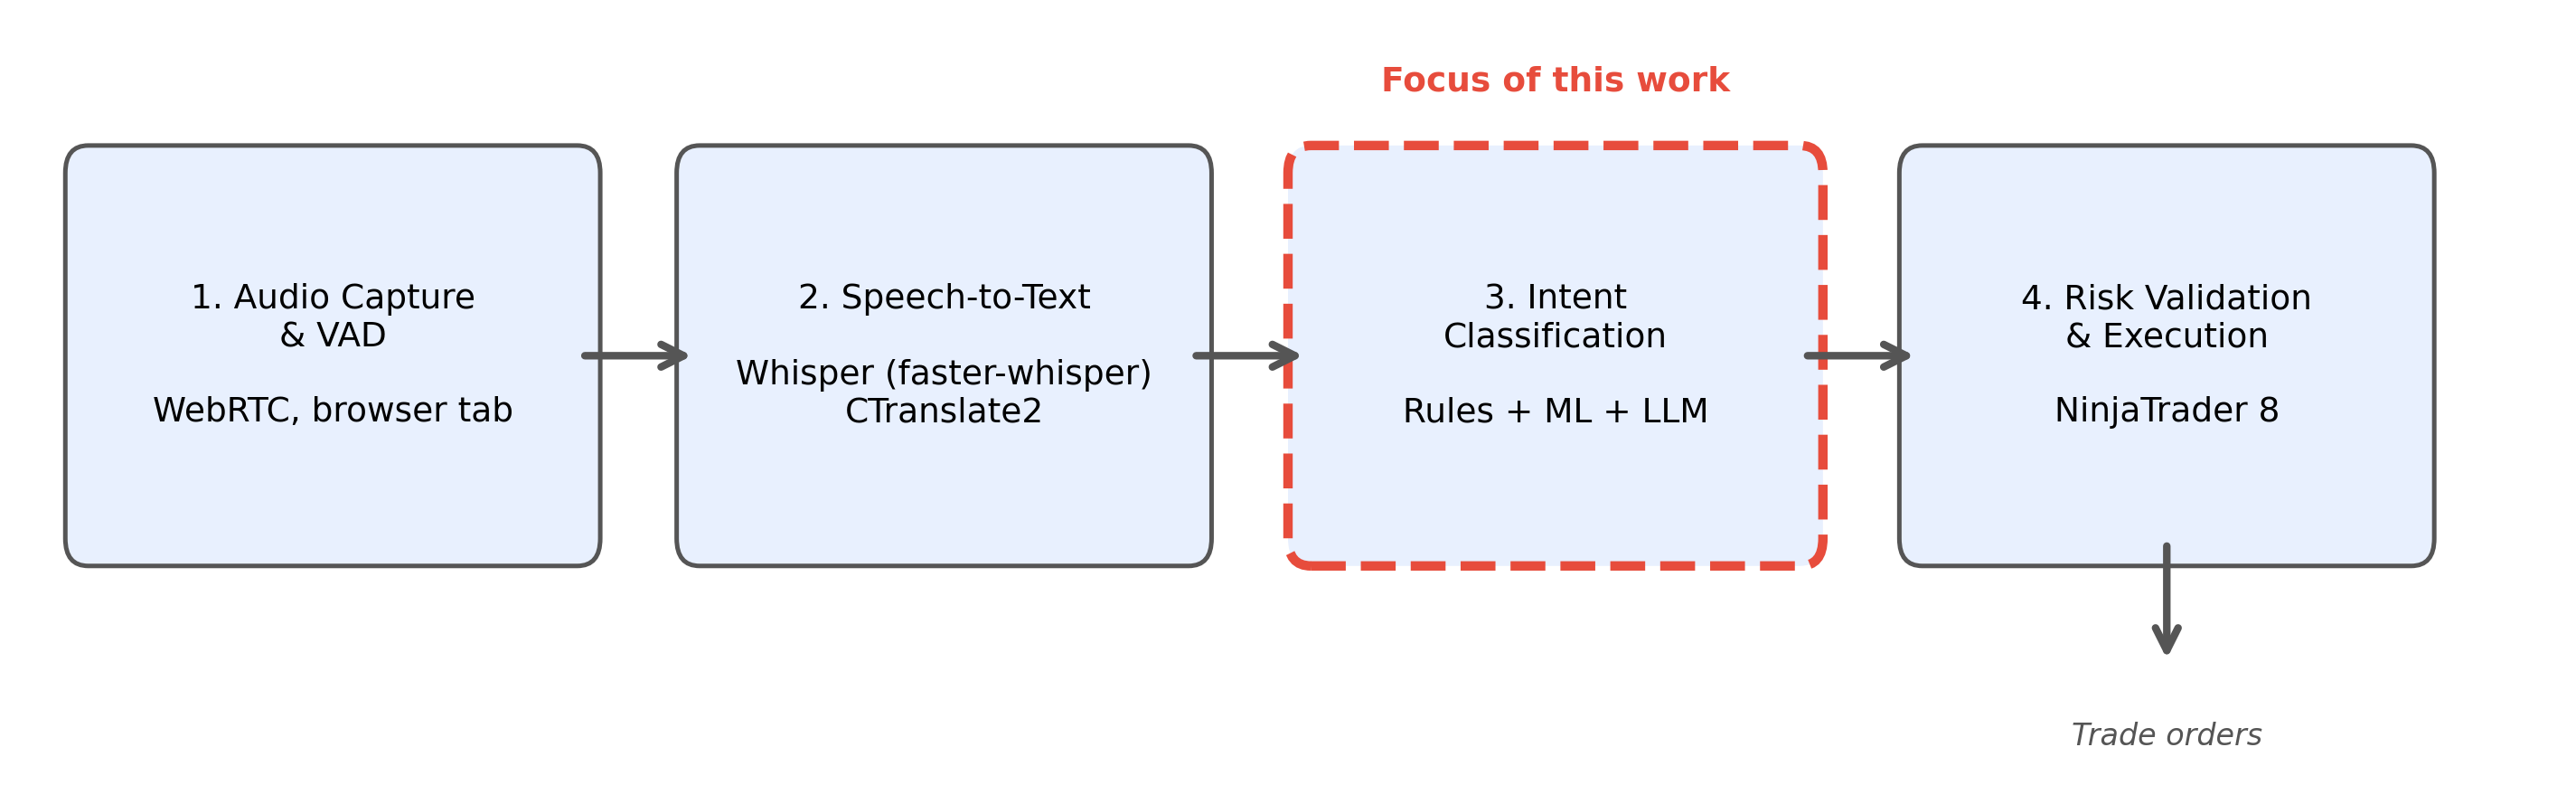
\includegraphics[width=0.95\textwidth]{pipeline.png}
\caption{Overview of the four-stage system pipeline. The classification stage (highlighted) is the component evaluated in this thesis. Audio is captured from a browser tab, transcribed by Whisper, classified into trading actions, and validated before execution.}
\label{fig:pipeline}
\end{figure}

\subsection{Task Definition and Label Set}
\label{sec:task_definition}

The classification task assigns one of seven labels to each input example. The labels and their definitions are shown in Table~\ref{tab:labels}.

\begin{table}[H]
\centering
\caption{Label definitions for the trade-intent classification task.}
\label{tab:labels}
\begin{tabularx}{\textwidth}{@{}llX@{}}
\toprule
\textbf{Label} & \textbf{Role} & \textbf{Description} \\
\midrule
\texttt{NO\_ACTION}          & Neutral    & No trade signal detected \\
\texttt{ENTER\_LONG}         & Entry      & Open a new long position \\
\texttt{ENTER\_SHORT}        & Entry      & Open a new short position \\
\texttt{TRIM}                & Management & Reduce position size (partial profit-taking) \\
\texttt{EXIT\_ALL}           & Management & Close the entire position \\
\texttt{MOVE\_STOP}          & Management & Adjust the stop-loss level \\
\texttt{MOVE\_TO\_BREAKEVEN} & Management & Move the stop-loss to the entry price \\
\bottomrule
\end{tabularx}
\end{table}

Each input example is a structured text prompt that encodes the traded instrument, the trader's current position state, and three overlapping windows of transcript text:

\begin{verbatim}
symbol=MNQ 03-26
position=LONG
last_side=LONG
recent=there s a nice shove up. we cleared out
analysis=there s a nice shove up. we cleared out there.
         so you got to take a partial
current=there. So, you got to take a partial
\end{verbatim}

The three text windows (\texttt{recent}, \texttt{analysis}, \texttt{current}) supply context at different temporal granularities, so the classifier sees not only the current utterance but also what was said just before; the \texttt{position} and \texttt{last\_side} fields encode the current market position, which is essential for telling management actions (which require an open position) from entry actions (which open one). The \texttt{symbol} field reads MNQ rather than NQ because the copying system executes its trades on the Micro E-mini Nasdaq contract (MNQ), a smaller-sized version of the NQ contract the streamer trades. This overlapping design addresses a core difficulty of streaming transcription: Whisper cuts audio into chunks of roughly 5--30 seconds, so a single utterance may be cut in half, and the overlap lets the classifier reconstruct the intent even when the decisive words are split across two lines.

Encoding the position state as plain text inside the prompt, rather than as a separate input, is done on purpose: it lets a single text-processing pipeline handle both the words and the trading context. How each model family digests these state lines is described in Section~\ref{sec:model_architectures}.

\subsection{Text Normalization}
\label{sec:normalization}

Between transcription and classification, a clean-up step corrects the recognition errors that occur most often in this domain, so that the classifier sees consistent text. It consists of 14 hand-written search-and-replace rules plus three general clean-ups, all applied as plain, deterministic text substitutions; no machine learning is involved.

A large share of the rules glues back together terms that Whisper tends to split apart. When the contract names that traders use as shorthand are spelled out letter by letter, ``m~n~q'' becomes ``mnq'' and ``e~s'' becomes ``es,'' and the price benchmark heard as ``v~w~a~p'' or even as ``view up'' becomes ``vwap.'' A second group of rules fixes sound-alike words in their trading sense, but only when the surrounding words make the trading meaning clear: a trader ``paying myself a peace'' is corrected to ``piece,'' and ``got my ad on'' becomes ``got my add on.'' Restricting these corrections to specific phrasings keeps the rules from corrupting genuine uses of the original words. A third group standardizes compounds that Whisper writes inconsistently, so ``break even'' and ``broke even'' both become ``breakeven,'' matching the spelling the labelled data uses. Finally, three general clean-ups run over everything: all text is lowercased, typographic apostrophes are replaced with plain ones, and the commas inside numbers are removed, so that a price like ``24,600'' is read as the single number ``24600'' rather than as two separate pieces.

Simple as they are, these substitutions reduce the vocabulary fragmentation caused by recognition errors: without them, ``vwap,'' ``v w a p,'' and ``view up'' would look like three unrelated expressions to the TF-IDF vectorizer and to the transformer tokenizers, even though the trader said the same word each time.

\subsection{Dataset Construction}
\label{sec:dataset_construction}

The training dataset was constructed in three stages: AI-assisted labelling, human review, and merging with normalization.

\textbf{Stage 1: AI labelling.} Trading livestream transcripts archived from YouTube were processed by large language models (LLMs), which assigned action labels to each transcript line based on the speaker's words and trading context. Three LLMs were used across different annotation passes: Claude Sonnet produced 278 labelled examples in an initial high-quality pass, Gemini Pro produced 78 examples in a validation run, and Gemini Flash produced 1.139 examples in a bulk labelling pass. This follows an idea from the research literature known as weak supervision: instead of having humans label every line, an automatic but imperfect labeller does the bulk of the work first, and humans then check and correct it~\cite{ratner2017snorkel}. Like any automated annotation, it makes mistakes: an LLM can mislabel sarcasm, hypothetical talk, or a half-finished sentence. The following stages catch many of these errors, but not all of them.

\textbf{Stage 2: Human review.} Each AI-generated label was manually reviewed by the author and either accepted, rejected, or corrected. Review decisions were preserved in the dataset as metadata fields, enabling downstream analysis of labelling reliability. This human-in-the-loop approach combines the scalability of automated labelling with the quality control of manual review, although review reduces errors rather than eliminating them.

\textbf{Stage 3: Merging and normalization.} The three reviewed collections were then combined into a single dataset; in the rare cases where two collections had labelled the same line, the newer label won. During the merge, two older label types were also translated into the final seven-label scheme. Lines where the trader merely talks about a possible future trade (``looking for shorts up here'') without acting were relabelled as \texttt{NO\_ACTION}, since they are commentary rather than an executed action; this affected 437 lines. And a handful of lines where the trader enlarges an existing position were converted into the matching entry label, because adding contracts is, from an execution standpoint, another entry in the same direction. The resulting dataset contains 1.466 examples drawn from 103 transcripts.

Two caveats apply to all of these labels. First, a label records what the trader \emph{announced}, not what verifiably happened: when a streamer says ``I'm long here,'' the dataset takes that entry at face value. No broker statements or account records were available, so there is no way to prove that an announced trade was actually placed. Second, although every label passed human review, the labels began as AI output, and the dataset cannot be assumed perfectly clean: the AI may have skipped real actions entirely, and since not every transcript was re-read line by line, such missed labels would go unnoticed. Both caveats are taken up again in Section~\ref{sec:limitations}.

\paragraph{Checking the labels by hand.}\label{sec:label_verification}
To see how far the labels can be trusted, they were also spot-checked. The 10 transcripts with the most action labels, around 200 labels in total, were re-read: for every labelled line, the surrounding lines were read to judge whether the label matches what the trader was actually doing at that moment. Almost every checked label held up, and none was clearly wrong. The same check, however, confirmed the missed-label problem from the other direction: the unlabelled lines of those same transcripts contain roughly 230 likely actions that carry no label, most of them repeats of an action announced moments earlier, small profit-takes, or stop adjustments mentioned in passing. In short, what is labelled is almost always right, but not everything that happened is labelled. Some lines labelled \texttt{NO\_ACTION} may therefore contain weak or repeated actions, which blurs the boundary between action and non-action during both training and evaluation. For this reason, the benchmark in this thesis should be read as a controlled comparison of models on the labelled examples, not as a measurement of how well trade signals are detected in raw livestream speech.

\subsection{Dataset Characteristics}
\label{sec:dataset_characteristics}

Table~\ref{tab:label_distribution} shows the label distribution of the original dataset.

\begin{table}[H]
\centering
\caption{Label distribution in the original dataset (1.466 file entries; 1.407 unique examples after content deduplication).}
\label{tab:label_distribution}
\begin{tabular}{@{}lrr@{}}
\toprule
\textbf{Label} & \textbf{Count} & \textbf{Percentage} \\
\midrule
\texttt{NO\_ACTION}          & 569 & 38,8\% \\
\texttt{TRIM}                & 267 & 18,2\% \\
\texttt{EXIT\_ALL}           & 271 & 18,5\% \\
\texttt{ENTER\_SHORT}        & 153 & 10,4\% \\
\texttt{MOVE\_STOP}          &  97 &  6,6\% \\
\texttt{ENTER\_LONG}         &  94 &  6,4\% \\
\texttt{MOVE\_TO\_BREAKEVEN} &  15 &  1,0\% \\
\midrule
\textbf{Total}               & \textbf{1.466} & \textbf{100\%} \\
\bottomrule
\end{tabular}
\end{table}

The distribution is strongly imbalanced, and it is worth being clear about where the \texttt{NO\_ACTION} examples come from. They are labelled lines like all the others: partly lines that the AI annotators explicitly marked as non-action commentary, and partly the 437 remapped setup lines described above. They are \emph{not} a random sample of all the chatter in the streams. That is why \texttt{NO\_ACTION} makes up only 38,8\% of this dataset, even though in a complete, uninterrupted session far more than 38,8\% of all spoken lines carry no action; compared to a real stream, the dataset is heavily \emph{action-enriched}. At the other extreme, \texttt{MOVE\_TO\_BREAKEVEN} has only 15 examples (1,0\%), far too few for any classifier to learn reliable patterns. Both points matter for interpreting all results and return in Sections~\ref{sec:label_verification} and~\ref{sec:limitations}.

\subsection{Data Cleanup}
\label{sec:data_cleanup}

Before model training, an automated cleanup pipeline corrected several recurring flaws in the original 1.466-example dataset.

The largest fix concerns contradictory position states. Some management-label examples (for example \texttt{TRIM} or \texttt{EXIT\_ALL}) carried \texttt{position=FLAT}, which is impossible: a trader cannot trim a position that does not exist. These contradictions survived the human review because the review judged whether the action label matched the trader's words; the position fields were filled in automatically during labelling and were not part of that check. In 200 examples, other recorded fields revealed the actual position and the state was repaired; the handful of contradictory examples that could not be repaired was removed.

The cleanup also removed two smaller groups. The first is repeated announcements: livestream speech repeats itself, so the same action sometimes ended up labelled twice within a few lines (``piece off into 50s'' and, two lines later, ``partial here, folks'' describe one single trim), and only the first occurrence was kept. The second is advice to the audience: a few lines address the viewers rather than describe the trader's own position (``you must pay yourself here''), and labelling those as executed trades would teach the classifier exactly the kind of false positive the system must avoid. After all steps, \textbf{1.442 clean examples} from 103 transcripts remain.

One last reduction happens automatically whenever the data is loaded: exact duplicates, entries whose label, prompt text, and position fields are all identical character for character, are collapsed into one. Such doubles arise because overlapping speech chunks can produce the very same prompt twice, and keeping both would let one line count twice in training and testing. This shrinks the original dataset from 1.466 to 1.407 unique examples, and the cleaned dataset from 1.442 to 1.377.

This gives four dataset sizes, which differ only by the two mechanical steps just described. Table~\ref{tab:dataset_sizes} lists them side by side.

\begin{table}[H]
\centering
\caption{The four dataset sizes used in this thesis. Each row differs from the row above by exactly one step: the cleanup removes 24 flawed examples, and loading the data collapses exact duplicates.}
\label{tab:dataset_sizes}
\small
\setlength{\tabcolsep}{4pt}
\begin{tabular}{@{}lcl@{}}
\toprule
\textbf{Stage} & \textbf{Examples} & \textbf{Role in this thesis} \\
\midrule
Raw merged dataset            & 1.466 & Input to the cleanup pipeline \\
After cleanup (24 removed)    & 1.442 & Cleaned dataset on disk \\
Raw, duplicates collapsed     & 1.407 & Baseline (Section~\ref{sec:results_original}) \\
Cleaned, duplicates collapsed & 1.377 & Primary results (Section~\ref{sec:results_cleaned}) \\
\bottomrule
\end{tabular}
\end{table}

All example counts and per-label support figures reported in Section~\ref{sec:results} refer to the deduplicated totals. The cleaned, deduplicated dataset (1.377 examples) is the primary basis for comparison; results on the original dataset are reported once, to measure the effect of cleanup.

\subsection{Model Architectures}
\label{sec:model_architectures}

This section describes how each model is set up. All models were implemented in Python, using scikit-learn~\cite{pedregosa2011scikit} for the classical models and the Hugging Face Transformers library~\cite{wolf2020transformers} with PyTorch~\cite{paszke2019pytorch} for the transformer models.

\subsubsection{TF-IDF Feature Extraction (Shared by Classical Models)}
\label{sec:tfidf_features}

All three classical models share the same text featurization step: TF-IDF vectorization with up to 20.000 features, consisting of unigrams and bigrams (single words and pairs of neighbouring words), with sublinear term-frequency scaling so that very frequent words do not dominate.

The effect is intuitive. A segment like \textit{``taking a partial here on this move up''} contains the bigram ``taking partial,'' which carries a high weight because it appears almost exclusively in \texttt{TRIM} examples, giving the classifier a strong signal. By contrast, \textit{``we got a nice shove up, let's try it''} contains no explicit trading keyword; phrases such as ``let's try'' appear across many classes and carry low weight, which is exactly why vaguely phrased entries are harder to classify than explicitly announced management actions.

The choice of 20.000 maximum features balances vocabulary coverage against dimensionality. With fewer than 1.500 training examples, a much larger vocabulary would mostly add features observed in only one or two examples, inviting overfitting. The inclusion of bigrams is particularly important for this domain: many trading actions are signalled by two-word phrases (``small long,'' ``move stop,'' ``I'm out,'' ``peel off'') that would be indistinguishable at the unigram level.

The structured prompt format means that the trading context is encoded by these same features. The vectorizer splits tokens at characters such as ``='', so a state line like \texttt{position=LONG} contributes the word pair ``position long'' as a bigram feature, and \texttt{position=FLAT} contributes ``position flat.'' Through these features, a model can learn, for example, that management actions go together with an open position; the feature-importance analysis later confirms that exactly these state bigrams carry substantial weight. In effect, the structured prompt turns a two-part problem (text plus trading state) into a single text classification problem that word-count features can handle.

\subsubsection{Logistic Regression}

Logistic regression is used as the first baseline, in the standard configuration of its scikit-learn implementation: a moderate amount of L2 regularization, so that no single word can dominate the decision, and balanced class weighting, so that the rare classes count more during training. It is the simplest model in the comparison, it outputs probabilities directly, and it handles the class imbalance out of the box.

\subsubsection{Support Vector Machine}

The linear SVM (\texttt{LinearSVC} in scikit-learn) uses the same feature vectors and the same balanced class weighting. Because an SVM produces only raw scores, the Platt-scaling step described earlier is trained on top of it to turn those scores into probabilities. The SVM draws its boundary to keep the widest possible margin between the classes, which can generalize better when training examples are scarce.

\subsubsection{Multi-Layer Perceptron}

The MLP is a two-layer feedforward neural network (hidden layers of 256 and 128 units) trained with the Adam optimizer~\cite{kingma2015adam}. Because scikit-learn's \texttt{MLPClassifier} cannot weight classes directly, balance is achieved by oversampling, and the mechanics are simple: every training example is duplicated in proportion to its balanced class weight. An example of the most common class appears once, while an example of a class that is, say, eight times rarer is copied about eight times, so the network simply sees the rare classes more often. Early stopping (halting training once performance on an internal validation split stops improving) is deliberately left off: the duplicated copies would land on both sides of that internal split, making the validation half look deceptively easy.

\subsubsection{DistilBERT (Frozen Encoder + Trained Head)}

The DistilBERT model (\texttt{distilbert-base-uncased}, 66 million parameters, 6 layers) is used as a frozen feature extractor~\cite{sanh2019distilbert}: the pretrained model itself is never changed and serves purely as a converter from text to numbers. The journey of one example is short, and Figure~\ref{fig:frozen_pipeline} shows it as a picture. The prompt text is first split into tokens. The frozen encoder then reads all tokens together and produces, for each one, a vector of 768 numbers describing that token in its context. These per-token vectors are averaged into a single vector of 768 numbers, a compact numerical summary of the whole example. Finally, that summary goes into the classification head, the only part that is trained: it rescales the 768 numbers to a stable range and computes one score per label, and the label with the highest score is the prediction.

\begin{figure}[H]
\centering
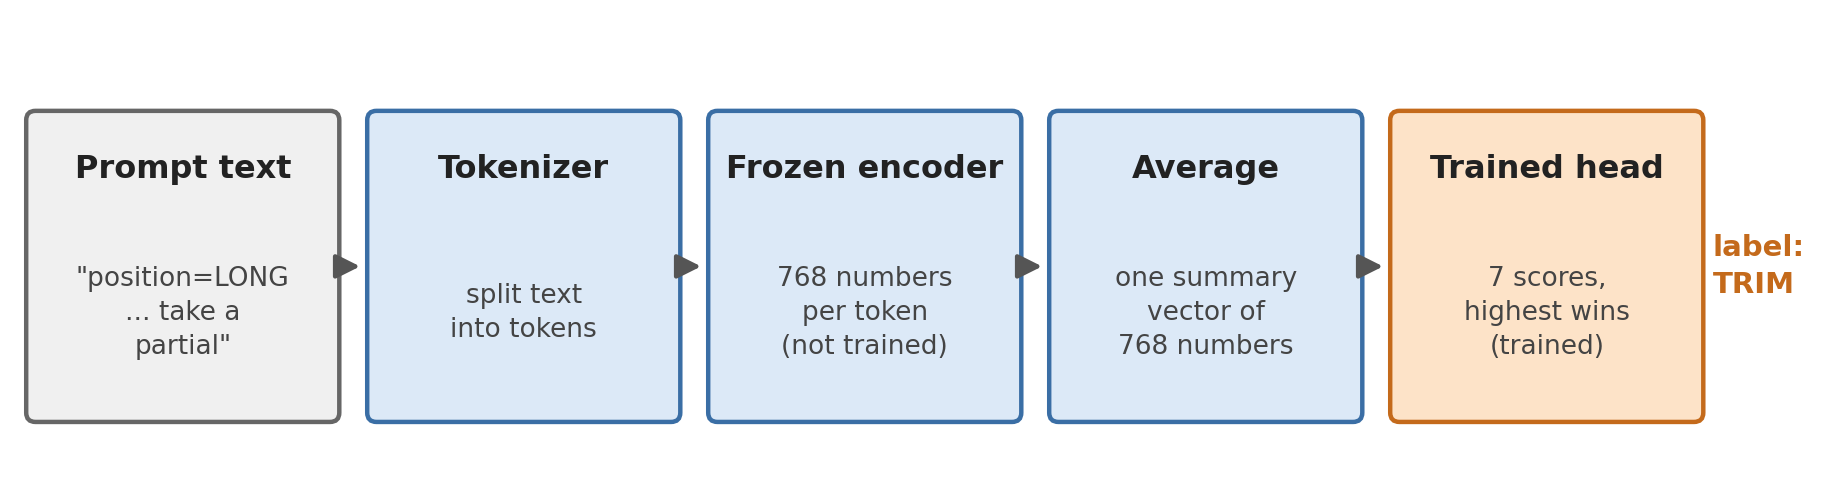
\includegraphics[width=0.95\textwidth]{frozen_encoder.png}
\caption{From text to prediction with a frozen encoder. Only the small classification head on the right is trained on the labelled data; the encoder stays exactly as pretrained.}
\label{fig:frozen_pipeline}
\end{figure}

The head is deliberately tiny: it contains only about 6.900 trainable parameters, against the 66 million frozen ones. It is trained like any small neural network, using the cross-entropy loss introduced earlier to measure how wrong the predictions are, with rare classes weighted more heavily so the head cannot ignore them, and an optimizer (AdamW~\cite{loshchilov2019decoupled}) that adjusts the 6.900 numbers over up to 20 passes through the training data.

Freezing the encoder is motivated by the small dataset. Full fine-tuning would mean adjusting 66 million parameters with only about 1.400 examples, roughly 45.000 adjustable numbers per example, and with that much freedom the model would mostly memorize the training set instead of learning patterns that transfer. Training only the head keeps the trained part at about five parameters per training example, which suits a controlled comparison on a corpus this size.

\subsubsection{ModernBERT (Frozen Encoder + Trained Head)}

The ModernBERT model (\path{answerdotai/ModernBERT-base}, 149 million parameters, 22 layers) is used in exactly the same way as DistilBERT: frozen encoder, averaged embeddings, and the identical trained head with the identical training procedure~\cite{warner2024modernbert}. The only difference is the encoder itself. ModernBERT has a newer design and was pretrained on far more text (about 2 trillion tokens, versus roughly 3,3 billion for the original BERT), so the 768-number summaries it produces should, in principle, capture meaning better. Whether they actually help on this task is precisely what the comparison measures: despite having more than twice DistilBERT's total parameters, ModernBERT has the same number of \emph{trainable} parameters here, since only the head is trained. Any advantage must come from the quality of its frozen embeddings.

\subsubsection{Model Comparison Summary}

Table~\ref{tab:model_summary} summarizes the key properties of all five models.

\begin{table}[H]
\centering
\caption{Summary of model architectures and key properties.}
\label{tab:model_summary}
\small
\setlength{\tabcolsep}{4pt}
\begin{tabularx}{\textwidth}{@{}lXXXX@{}}
\toprule
\textbf{Model} & \textbf{Total parameters} & \textbf{Input representation} & \textbf{Task-trained parameters} & \textbf{Class-imbalance handling} \\
\midrule
Logistic regression & $\sim$140.000 & TF-IDF, up to 20.000 features & All & Balanced class weights \\
Linear SVM & $\sim$140.000 & TF-IDF, up to 20.000 features & All & Balanced class weights \\
Multi-layer perceptron & $\sim$5,4 million & TF-IDF, up to 20.000 features & All & Balanced oversampling \\
DistilBERT frozen head & 66 million + 6.900 & Token sequence & Head only (6.900) & Weighted loss \\
ModernBERT frozen head & 149 million + 6.900 & Token sequence & Head only (6.900) & Weighted loss \\
\bottomrule
\end{tabularx}
\end{table}

One contrast in this table is worth spelling out, because it shapes the results. The classical models train every one of their parameters on the task: logistic regression, for example, can adjust up to 140.000 weights (7 classes $\times$ 20.000 features), of which roughly half are active once the actual vocabulary saturates at about 10.000 features (Section~\ref{sec:vocab_ablation}). The transformers, by contrast, keep more than 99,99\% of their parameters frozen and adapt only the 6.900 weights of the head. So although the transformers are vastly bigger models overall, the part that can actually specialize in trading language is about an order of magnitude \emph{smaller} than in the classical models. How much this matters is examined in the results and the discussion.

\subsection{Evaluation Protocol}
\label{sec:evaluation}

\subsubsection{Cross-Validation with Transcript-Level Splits}

With fewer than 1.500 labelled examples, holding out one fixed test set would be wasteful and fragile: much of the scarce data would be locked away from training, and the result would depend on which lines happen to land in the held-out set. The standard way around this is \emph{cross-validation}~\cite{kohavi1995study}. The data is split into five parts, called folds. The models are then trained five times, each time on four of the parts, and tested on the remaining fifth. Every example is therefore used for testing exactly once, always by a model that never saw it during training, and the five test scores are averaged. All models in this thesis are evaluated this way.

One detail of the split is critical. In standard cross-validation, individual examples are shuffled randomly into folds. That is fine for unrelated examples, but the examples here are not unrelated: lines from the same transcript share the same speaker, the same market day, the same audio quality, and verbal habits that recur throughout a session. If lines from one transcript landed in both the training and the test set, a model could score well partly by recognizing the session rather than understanding the language, and the measured accuracy would be too optimistic. This effect is known as data leakage. To rule it out, entire transcripts are assigned to folds, never single lines, so a model is always tested on sessions it has never seen. The assignment itself is deterministic (it uses a fixed hash of each transcript's file path), so every rerun produces the same folds. The 103 transcripts spread across the 5 folds with roughly 20 transcripts each, though the number of examples per fold varies with how long each session ran and how actively the trader traded in it (exact figures in Section~\ref{sec:reproducibility}).

Within each fold, the training set is rebalanced by downsampling \texttt{NO\_ACTION} examples, so that their number does not exceed 2,5 times the total number of action examples. The choice of which \texttt{NO\_ACTION} examples to keep is made by sorting them by a fixed scrambling code (a hash) of each example's identity and keeping the first ones; this behaves like a random draw but produces exactly the same selection on every rerun. The downsampling applies only to the training part of each fold; the test part keeps the proportions of the labelled dataset. Because the dataset is action-enriched (Section~\ref{sec:label_verification}), these proportions should not be read as the true frequency of action and non-action speech in an uninterrupted livestream.

\subsubsection{Metrics}
\label{sec:metrics}

Five metrics are reported, following established practice for imbalanced multi-class classification~\cite{sokolova2009systematic}.

\textbf{Accuracy} is the fraction of correctly classified examples. It is simple but can mislead on imbalanced data: a classifier that always predicts \texttt{NO\_ACTION} would reach about 39\% accuracy here without detecting a single trade.

\textbf{Macro F1} is the unweighted mean of the per-class F1 scores, treating all seven classes equally. A model that ignores the rare classes is punished visibly by this metric, which makes it a more balanced assessment than accuracy. The F1 score itself is the harmonic mean of precision and recall:

\begin{equation}
F_1 = 2 \cdot \frac{\text{Precision} \times \text{Recall}}{\text{Precision} + \text{Recall}}
\label{eq:f1}
\end{equation}

\textbf{Action F1}, the primary metric, reduces the problem to one binary question: did the system recognize that \emph{some} trade action occurred? Any action prediction on an action example counts as a true positive; an action prediction on a \texttt{NO\_ACTION} example is a false positive; a \texttt{NO\_ACTION} prediction on an action example is a false negative. This directly measures the system's ability to separate actionable signals from commentary, which is its central job.

\textbf{Action precision} is the fraction of all action predictions that were truly actions; high precision means few false alarms. \textbf{Action recall} is the fraction of all true actions that were predicted as some action; high recall means few missed signals.

One more term appears throughout the result tables: the \emph{support} of a class is simply the number of test examples whose true label is that class. It says how much evidence stands behind each per-class score; a score computed over 13 examples (as for \texttt{MOVE\_TO\_BREAKEVEN}) is far less stable than one computed over 548.

\subsubsection{Benchmark Artifacts}
\label{sec:reproducibility}

All results in this thesis are read from stored result files written by the benchmark scripts, and the repository contains all of the code needed to regenerate them. The underlying data is a different matter: the labelled dataset and the full transcript archive are too large for the public repository, so only five example transcripts are included to show the data format. An outside reader can therefore inspect every piece of code and every stored result, but rerunning the experiments requires building a dataset of one's own.

Inside the pipeline, two safeguards matter most. The TF-IDF vocabulary is learned inside each training fold only and never from test data, and all splits and seeds are fixed, so reruns produce the same folds (only the transformer heads can vary minimally between reruns, due to random initialization).

Across the five folds, the split assigns 21, 21, 21, 21, and 19 transcripts (225, 339, 287, 293, and 233 test examples, respectively), for 1.377 examples in total. Table~\ref{tab:support} lists how often each label occurs among these test examples, summed over all folds; these are the support columns of the per-label tables in Section~\ref{sec:results_per_label}.

\begin{table}[H]
\centering
\caption{Per-label support: the number of test examples per class on the cleaned dataset, summed across all five folds.}
\label{tab:support}
\begin{tabular}{@{}lr@{}}
\toprule
\textbf{Label} & \textbf{Support} \\
\midrule
\texttt{NO\_ACTION}          & 548 \\
\texttt{EXIT\_ALL}           & 244 \\
\texttt{TRIM}                & 242 \\
\texttt{ENTER\_SHORT}        & 144 \\
\texttt{MOVE\_STOP}          &  94 \\
\texttt{ENTER\_LONG}         &  92 \\
\texttt{MOVE\_TO\_BREAKEVEN} &  13 \\
\bottomrule
\end{tabular}
\end{table}


% ═══════════════════════════════════════════════════════════════
% 4. RESULTS
% ═══════════════════════════════════════════════════════════════
\section{Results}
\label{sec:results}

This section presents the results in three parts. First come the main scores of all five models on the cleaned dataset, together with a comparison against the uncleaned dataset that shows what the cleanup was worth. The middle subsections then take the results apart to understand them: scores per label, the typical confusions, which words drive the decisions, statistical tests, and an error analysis. Finally, the last two subsections leave the labelled dataset behind and test the system on five complete livestream sessions, first the best model on its own and then the full production pipeline.

\subsection{Primary Results on the Cleaned Dataset}
\label{sec:results_cleaned}

Table~\ref{tab:results_cleaned} presents the five-fold cross-validation results on the cleaned dataset (1.377~unique examples after content deduplication, 103~transcripts). Values are reported as mean $\pm$ standard deviation across folds. For this primary evaluation, the MLP uses the balanced oversampling procedure described in Section~\ref{sec:model_architectures}.

\begin{table}[H]
\centering
\caption{Five-fold cross-validation results on the cleaned dataset (primary evaluation). Bold indicates best per column.}
\label{tab:results_cleaned}
\footnotesize
\setlength{\tabcolsep}{2pt}
\begin{tabular}{@{}lccccc@{}}
\toprule
\textbf{Model} & \textbf{Accuracy} & \textbf{Macro F1} & \textbf{Action F1} & \shortstack{\textbf{Action}\\\textbf{precision}} & \shortstack{\textbf{Action}\\\textbf{recall}} \\
\midrule
Linear SVM          & \textbf{0,795}{\scriptsize$\pm$0,021} & 0,688{\scriptsize$\pm$0,062} & 0,884{\scriptsize$\pm$0,011} & \textbf{0,900}{\scriptsize$\pm$0,031} & 0,870{\scriptsize$\pm$0,020} \\
Logistic regression & 0,785{\scriptsize$\pm$0,021} & \textbf{0,703}{\scriptsize$\pm$0,045} & \textbf{0,887}{\scriptsize$\pm$0,024} & 0,863{\scriptsize$\pm$0,033} & 0,914{\scriptsize$\pm$0,024} \\
MLP                 & 0,763{\scriptsize$\pm$0,024} & 0,634{\scriptsize$\pm$0,049} & 0,850{\scriptsize$\pm$0,006} & 0,898{\scriptsize$\pm$0,037} & 0,809{\scriptsize$\pm$0,031} \\
ModernBERT          & 0,727{\scriptsize$\pm$0,012} & 0,649{\scriptsize$\pm$0,060} & 0,872{\scriptsize$\pm$0,031} & 0,833{\scriptsize$\pm$0,044} & \textbf{0,917}{\scriptsize$\pm$0,037} \\
DistilBERT          & 0,676{\scriptsize$\pm$0,065} & 0,588{\scriptsize$\pm$0,029} & 0,848{\scriptsize$\pm$0,034} & 0,801{\scriptsize$\pm$0,070} & 0,909{\scriptsize$\pm$0,071} \\
\bottomrule
\end{tabular}
\end{table}

The two linear classical models achieve the strongest aggregate performance. Logistic regression reaches the best macro F1 (0,703) and action F1 (0,887), while the SVM reaches the best accuracy (0,795) and action precision (0,900). ModernBERT has the highest action recall (0,917), but this comes with lower precision and lower macro F1. The MLP, after balanced oversampling, occupies a middle position: it is more conservative than the transformers and less accurate than the two linear models.

\subsection{Original Dataset Baseline and Cleanup Effects}
\label{sec:results_original}

To quantify the impact of data cleanup, every model was also evaluated on the original dataset (1.407 unique examples after content deduplication, 103~transcripts) using the same protocol. These original-dataset scores serve only as a secondary baseline and are not used for the per-label and error analyses; rather than reproduce all five rows here, the effect of cleanup is reported directly as a difference. Table~\ref{tab:cleanup_delta} gives, for each model, the change in the three central metrics (cleaned minus original). For the MLP, the unbalanced configuration is used on both datasets, so the cleanup effect is not mixed with the separate balancing change.

\begin{table}[H]
\centering
\caption{Cleanup-only performance change (cleaned minus original). Positive values indicate improvement. The MLP row uses the unbalanced MLP configuration on both datasets, so the cleanup effect is not mixed with the later balancing change.}
\label{tab:cleanup_delta}
\begin{tabular}{@{}lccc@{}}
\toprule
\textbf{Model} & \textbf{$\Delta$ Accuracy} & \textbf{$\Delta$ Macro F1} & \textbf{$\Delta$ Action F1} \\
\midrule
Linear SVM          & +0,020 & +0,017 & +0,014 \\
Logistic regression & +0,022 & +0,024 & +0,016 \\
ModernBERT          & +0,048 & +0,047 & +0,017 \\
DistilBERT          & +0,038 & $-$0,006 & +0,011 \\
MLP (unbalanced)    & $-$0,006 & $-$0,019 & $-$0,005 \\
\bottomrule
\end{tabular}
\end{table}

Cleanup improved most model metrics. ModernBERT gained +0,048 accuracy and +0,047 macro F1, compared to +0,022 and +0,024 for logistic regression. DistilBERT improved in accuracy and action F1 but decreased slightly in macro F1. The unbalanced MLP did not benefit from cleanup alone, which indicates that its earlier weakness was driven more by class-imbalance handling than by the specific noisy examples removed during cleanup. The separate effect of balanced oversampling on the MLP (Section~\ref{sec:mlp_balanced}) is sizeable: on the same cleaned dataset it raises accuracy from 0,726 to 0,763, macro F1 from 0,572 to 0,634, and action F1 from 0,804 to 0,850. The gains from cleanup are modest in absolute terms, but they make the classic point of garbage in, garbage out: the same models, given slightly cleaner data, learn measurably better.

\subsection{Per-Label Performance}
\label{sec:results_per_label}

Table~\ref{tab:per_label_linear} shows the per-label precision, recall, and F1 for the two linear models on the cleaned dataset, aggregated across all five folds.

\begin{table}[H]
\centering
\caption{Per-label precision (P), recall (R), and F1 for the two TF-IDF linear models on the cleaned dataset. Supp.\ = support, the number of test examples whose true label is the class in question.}
\label{tab:per_label_linear}
\small
\setlength{\tabcolsep}{4pt}
\begin{tabular}{@{}l ccc ccc c@{}}
\toprule
& \multicolumn{3}{c}{\textbf{Logistic regression}} & \multicolumn{3}{c}{\textbf{Linear SVM}} & \\
\cmidrule(lr){2-4}\cmidrule(lr){5-7}
\textbf{Label} & \textbf{P} & \textbf{R} & \textbf{F1} & \textbf{P} & \textbf{R} & \textbf{F1} & \textbf{Supp.} \\
\midrule
\texttt{NO\_ACTION}          & 0,857 & 0,777 & 0,815 & 0,812 & 0,850 & 0,831 & 548 \\
\texttt{ENTER\_LONG}         & 0,574 & 0,717 & 0,638 & 0,684 & 0,587 & 0,632 &  92 \\
\texttt{ENTER\_SHORT}        & 0,614 & 0,618 & 0,616 & 0,676 & 0,521 & 0,588 & 144 \\
\texttt{TRIM}                & 0,786 & 0,835 & 0,810 & 0,797 & 0,860 & 0,827 & 242 \\
\texttt{EXIT\_ALL}           & 0,811 & 0,861 & 0,835 & 0,829 & 0,857 & 0,843 & 244 \\
\texttt{MOVE\_STOP}          & 0,818 & 0,862 & 0,839 & 0,833 & 0,851 & 0,842 &  94 \\
\texttt{MOVE\_TO\_BREAKEVEN} & 0,800 & 0,308 & 0,444 & 0,750 & 0,231 & 0,353 &  13 \\
\bottomrule
\end{tabular}
\end{table}

A clear hierarchy of difficulty emerges. Management labels (\texttt{TRIM}, \texttt{EXIT\_ALL}, \texttt{MOVE\_STOP}) achieve F1 scores between 0,810 and 0,839, reflecting the use of explicit, distinctive keywords (``partial,'' ``taking profit,'' ``I'm out,'' ``move my stop''). Entry labels (\texttt{ENTER\_LONG}, \texttt{ENTER\_SHORT}) are considerably harder, with F1 scores around 0,62--0,64, because entry language is more varied and ambiguous (``let's try it,'' ``here we go,'' ``small size long here''). The rarest class, \texttt{MOVE\_TO\_BREAKEVEN}, improves to F1~=~0,444 after cleanup but still has only 13 support examples, too few for reliable learning.

The SVM shows the same overall pattern but trades off differently on the entry classes. It is right more often when it does call an entry (precision 0,684 on \texttt{ENTER\_LONG}, versus 0,574 for logistic regression), but it calls far fewer of them (recall 0,587 versus 0,717). In plain terms, the SVM only announces an entry when the wording is unmistakable, which makes it more cautious than logistic regression on exactly the classes where wording varies most.

\subsection{Transformer Model Performance}
\label{sec:results_transformers}

Table~\ref{tab:per_label_transformers} presents the per-label results for the two transformer models side by side.

\begin{table}[H]
\centering
\caption{Per-label precision (P), recall (R), and F1 for the two frozen transformer models on the cleaned dataset. Supp.\ = support, the number of test examples whose true label is the class in question.}
\label{tab:per_label_transformers}
\small
\setlength{\tabcolsep}{4pt}
\begin{tabular}{@{}l ccc ccc c@{}}
\toprule
& \multicolumn{3}{c}{\textbf{DistilBERT}} & \multicolumn{3}{c}{\textbf{ModernBERT}} & \\
\cmidrule(lr){2-4}\cmidrule(lr){5-7}
\textbf{Label} & \textbf{P} & \textbf{R} & \textbf{F1} & \textbf{P} & \textbf{R} & \textbf{F1} & \textbf{Supp.} \\
\midrule
\texttt{NO\_ACTION}          & 0,825 & 0,637 & 0,719 & 0,855 & 0,712 & 0,777 & 548 \\
\texttt{ENTER\_LONG}         & 0,441 & 0,565 & 0,495 & 0,516 & 0,533 & 0,524 &  92 \\
\texttt{ENTER\_SHORT}        & 0,436 & 0,542 & 0,483 & 0,497 & 0,611 & 0,548 & 144 \\
\texttt{TRIM}                & 0,651 & 0,756 & 0,700 & 0,714 & 0,826 & 0,766 & 242 \\
\texttt{EXIT\_ALL}           & 0,720 & 0,738 & 0,729 & 0,709 & 0,771 & 0,739 & 244 \\
\texttt{MOVE\_STOP}          & 0,681 & 0,862 & 0,761 & 0,821 & 0,830 & 0,825 &  94 \\
\texttt{MOVE\_TO\_BREAKEVEN} & 0,429 & 0,231 & 0,300 & 0,667 & 0,462 & 0,546 &  13 \\
\bottomrule
\end{tabular}
\end{table}

Both frozen transformer feature extractors show lower precision on entry classes than the two linear models. DistilBERT achieves 0,441 precision on \texttt{ENTER\_LONG} (versus 0,574 for logistic regression), while ModernBERT reaches 0,516. The transformers do achieve relatively high recall on several action classes; DistilBERT detects 86,2\% of \texttt{MOVE\_STOP} actions, but the frequency of false positives lowers their macro F1.

ModernBERT achieves the highest F1 on \texttt{MOVE\_TO\_BREAKEVEN} (0,546) of all five models, despite the extreme rarity of this class. This suggests that its contextual embeddings capture some similarity between ``breakeven'' language and other stop-management language, although this advantage on one rare label does not translate into the best aggregate score.

Across all five models, the per-label F1 scores follow the same difficulty hierarchy: management labels are classified reliably, entry labels are consistently harder and vary more between models, and \texttt{MOVE\_TO\_BREAKEVEN} remains unstable with only 13 support examples.

\subsection{Confusion Matrix Analysis}
\label{sec:confusion_matrices}

A confusion matrix is the most direct way to see what kinds of mistakes a model makes. Each row collects the examples whose true label is the row's class, and each column shows which label the model predicted. Correct predictions therefore lie on the diagonal, and every off-diagonal cell counts one specific kind of error. Figure~\ref{fig:cm} shows the confusion matrices for logistic regression, the best model by macro F1 and action F1, and for ModernBERT, the stronger of the two transformers, both aggregated across all five folds on the cleaned dataset.

\begin{figure}[H]
\centering
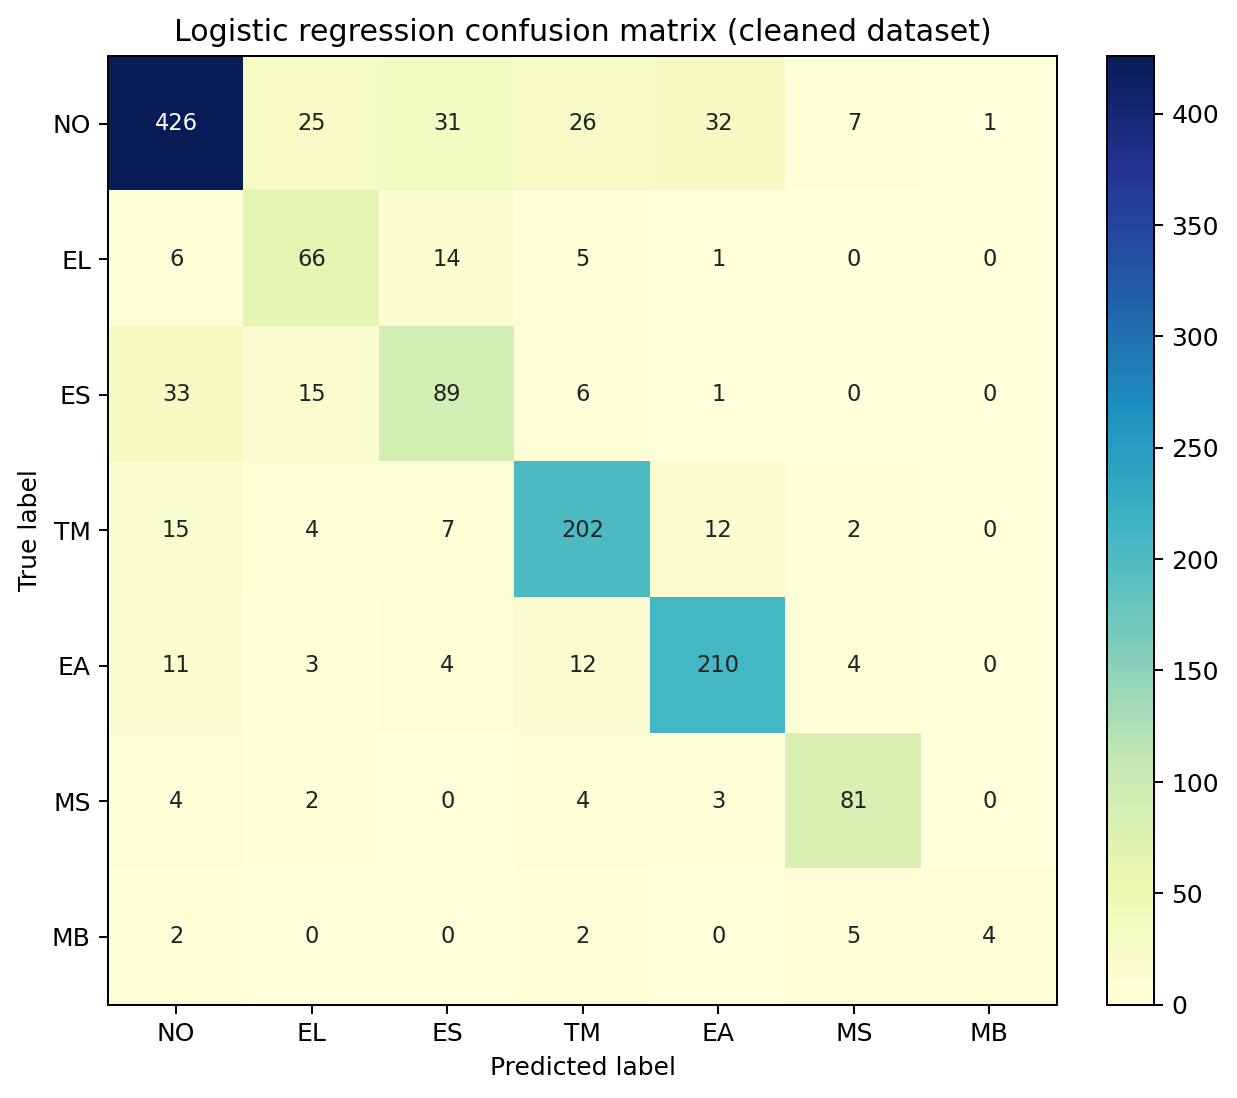
\includegraphics[width=0.49\textwidth]{confusion_matrix.png}\hfill
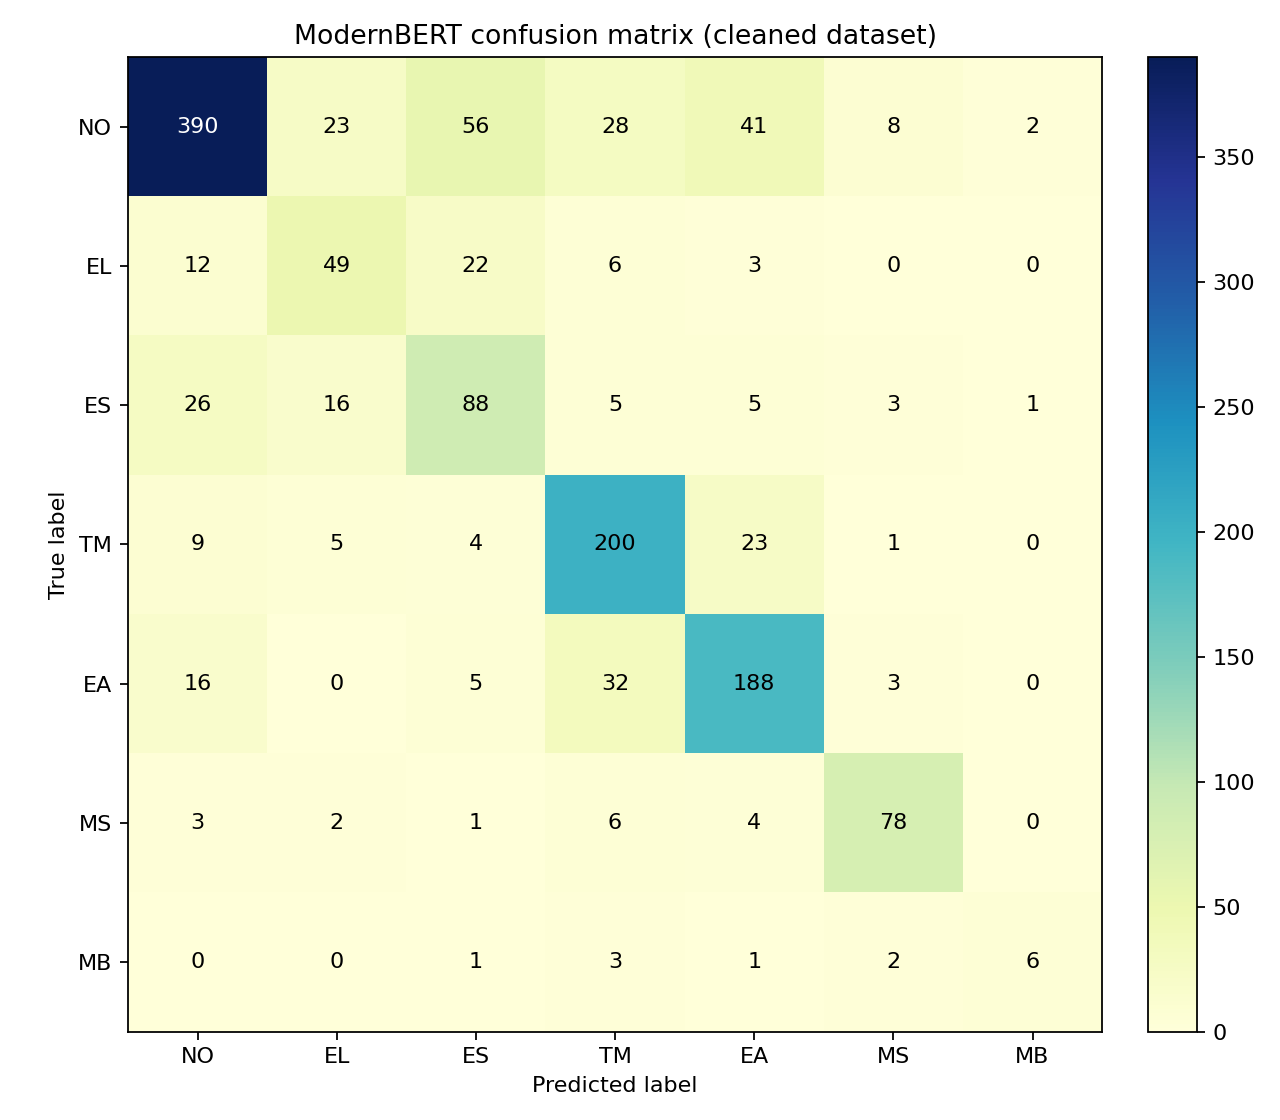
\includegraphics[width=0.49\textwidth]{confusion_matrix_modernbert.png}
\caption{Confusion matrices for logistic regression (left) and ModernBERT (right) on the cleaned dataset, aggregated across all five folds. Rows are true labels, columns are predicted labels, so the diagonal counts correct predictions; darker cells contain more examples. NO = \texttt{NO\_ACTION}, EL = \texttt{ENTER\_LONG}, ES = \texttt{ENTER\_SHORT}, TM = \texttt{TRIM}, EA = \texttt{EXIT\_ALL}, MS = \texttt{MOVE\_STOP}, MB = \texttt{MOVE\_TO\_BREAKEVEN}.}
\label{fig:cm}
\end{figure}

Several error patterns stand out in the logistic regression matrix.

\textbf{Confusing the direction of an entry.} 14 of 92 true \texttt{ENTER\_LONG} examples are misclassified as \texttt{ENTER\_SHORT}; conversely, 15 of 144 true \texttt{ENTER\_SHORT} examples are misclassified as \texttt{ENTER\_LONG}. Entry language is often structurally similar regardless of direction, differing only in a directional keyword (``long'' versus ``short'') that may be transcribed ambiguously or may be missing from the relevant text window.

\textbf{Missed actions.} Between 2 and 33 examples of each action class are misclassified as \texttt{NO\_ACTION}. This happens when the transcript contains an action but the language is too subtle for the classifier, for example a trader who says ``I'm going to take a little off'' rather than using the explicit keyword ``partial.''

\textbf{False alarms.} 122 of 548 \texttt{NO\_ACTION} examples (22,3\%) are assigned an action label. Some non-action segments contain language that superficially resembles action language, for example when the trader discusses a hypothetical trade, reviews a past action, or gives advice to viewers. Because the corpus has incomplete action coverage (Section~\ref{sec:label_verification}), a small number of these apparent false positives may also be genuinely unlabelled actions. The rare \texttt{MOVE\_TO\_BREAKEVEN} class barely registers in these totals; with 13 examples it stays unstable, and its most frequent error, landing on \texttt{MOVE\_STOP}, is at least the most closely related class.

The ModernBERT matrix (right panel) shows the opposite tendency. Logistic regression classifies 426 of the 548 \texttt{NO\_ACTION} examples correctly; ModernBERT manages only 390 and DistilBERT only 349, because both more often place a non-action line into one of the action columns. In other words, when the frozen transformers are unsure, they lean towards predicting an action. That is exactly why their action recall is high and their precision low in Table~\ref{tab:results_cleaned}: they catch more of the real actions, but they also raise more false alarms. The two remaining models lean the other way: the SVM behaves like a stricter logistic regression, and the balanced MLP is the most conservative of all, sending 27 true \texttt{ENTER\_LONG} and 50 true \texttt{ENTER\_SHORT} examples to \texttt{NO\_ACTION}.

\subsection{Feature Importance Analysis}
\label{sec:feature_importance}

To understand \emph{why} TF-IDF-based models do so well, the learned logistic regression weights were inspected directly. The ranking considers every feature the model uses, single words and two-word phrases alike. Figure~\ref{fig:feature_importance} shows the five highest-weighted features for three representative action classes.

\begin{figure}[H]
\centering
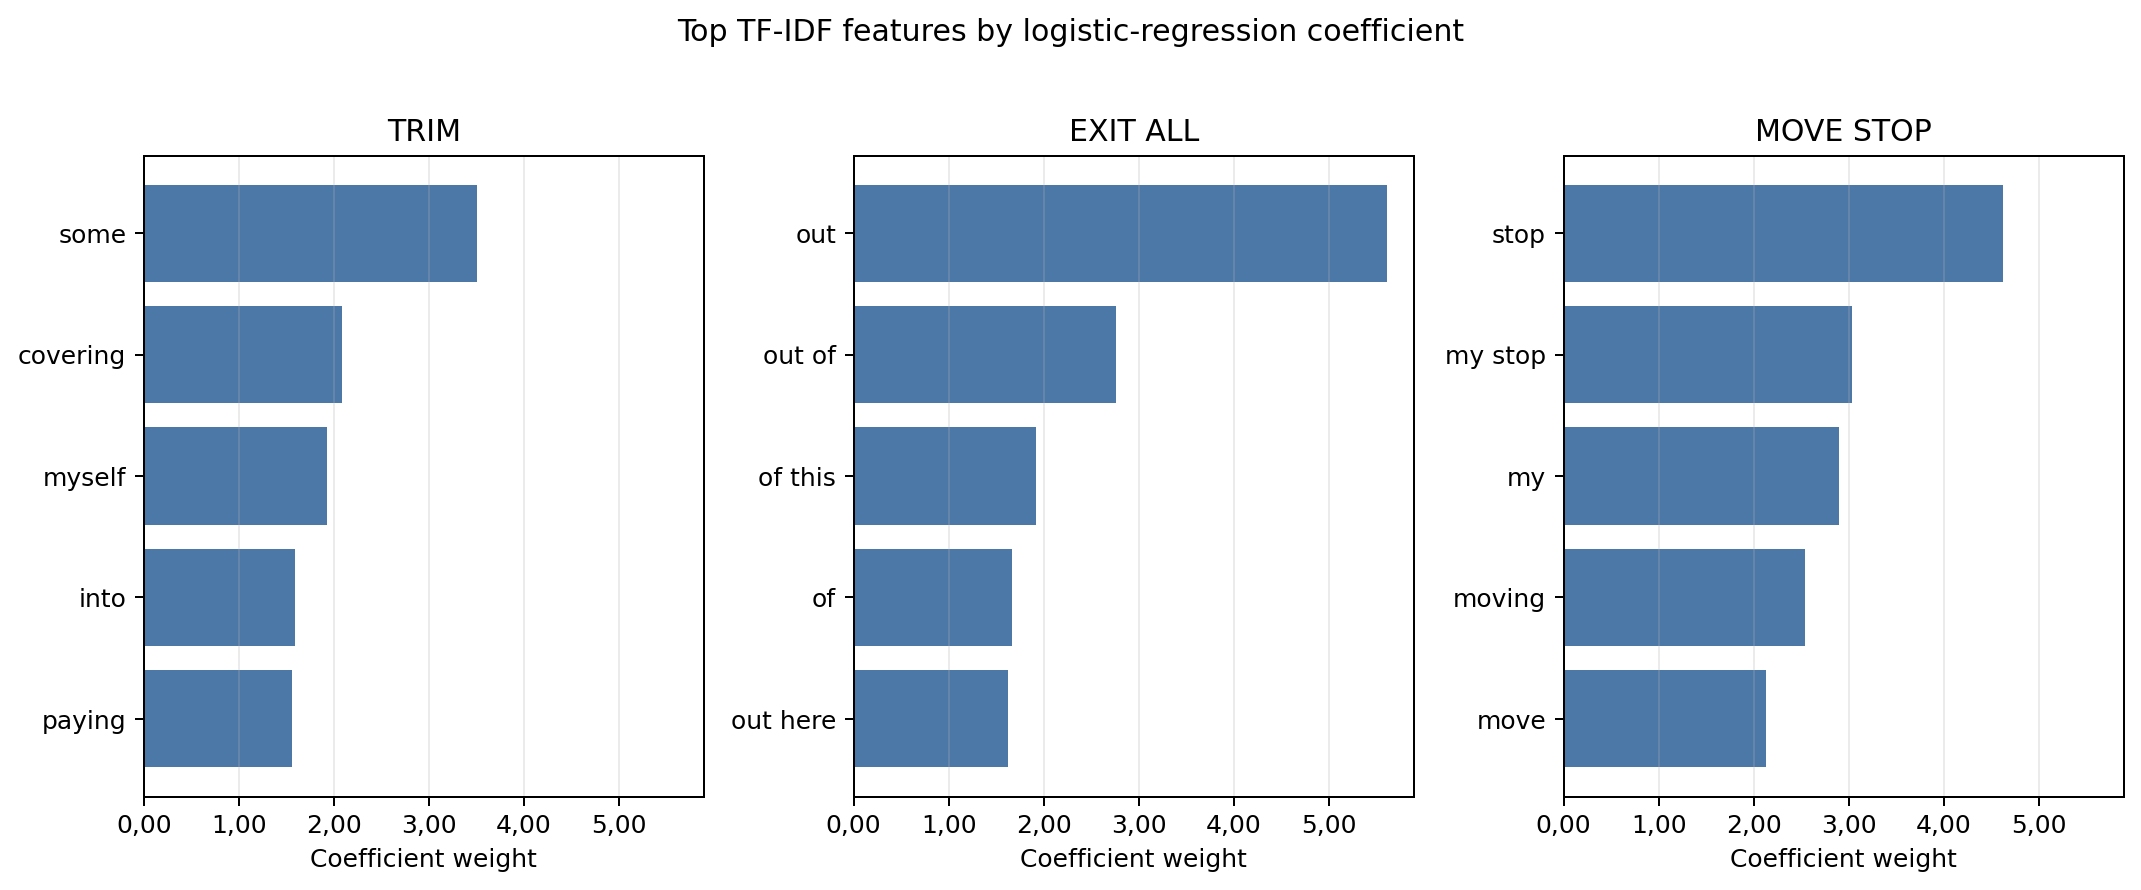
\includegraphics[width=0.85\textwidth]{feature_importance.png}
\caption{Top-5 TF-IDF features by logistic regression coefficient for three action classes. Each subplot shows the five most predictive words or bigrams for one class. A single token (``out'') dominates \texttt{EXIT\_ALL} with weight +5,61, while ``stop'' dominates \texttt{MOVE\_STOP} at +4,62. All subplots share the same x-axis scale, making the relative dominance of top features directly comparable across classes.}
\label{fig:feature_importance}
\end{figure}

The feature weights reveal that trading action language is built from a small set of fixed, recurring phrases. \texttt{EXIT\_ALL} is dominated by the single word ``out'' (weight +5,61); \texttt{MOVE\_STOP} by ``stop'' (+4,62); \texttt{TRIM} by ``some'' (+3,51). These sparse, high-signal features are captured directly by TF-IDF, whereas in a frozen transformer embedding the same keywords are blended with everything else in the segment into one dense 768-number summary, where their signal is diluted. The position-state bigrams (``position flat,'' ``position short'') also carry high weight, confirming that the structured prompt design (Section~\ref{sec:task_definition}) contributes real classification signal.

\subsection{Statistical Significance}
\label{sec:significance}

Mean scores alone do not show whether a difference between two models is real or just luck with the particular folds. A standard check is the paired $t$-test: for two models scored on the same five folds, it asks whether the per-fold differences point consistently in one direction or could plausibly be chance. Its output, the $p$-value, is the probability of seeing differences at least this large if the models were actually equally good; by convention, values below 0,05 count as evidence of a real difference. With only five folds these tests have little power, meaning only large and consistent differences can reach significance, so they are reported as a sanity check rather than as proof.

Each pair of models was compared with such a test on its per-fold macro F1 scores, using the same model versions as Table~\ref{tab:results_cleaned} (for the MLP, the balanced one). These pairwise comparisons ask the natural question of this benchmark: is model A really better than model B, or only on average? The answer is sobering. The two linear models are statistically indistinguishable ($p = 0{,}54$), and neither separates significantly from the balanced MLP. Of the classical-versus-transformer comparisons, only logistic regression versus DistilBERT reaches conventional significance ($p = 0{,}014$); the comparisons with ModernBERT do not. (One technical note: when many tests are run at once, a few can look significant purely by chance, a problem known as multiple comparisons. No correction for it is applied here, since with six tests, of which five are negative anyway, it would not change the picture.)

Looking at the individual folds shows why the tests stay cautious: the linear models win on average, but ModernBERT takes the best macro F1 in one fold, and the transformers take the best action recall in several. The fair summary is that the linear models are ahead overall, and the feature-importance and embedding analyses explain why, but the gap is not so large that it shows up consistently in every single fold.

\subsection{MLP Performance with Balanced Class Weighting}
\label{sec:mlp_balanced}

The unbalanced MLP fails entirely on \texttt{MOVE\_TO\_BREAKEVEN} (F1~=~0,000) and depresses minority-class recall; balanced oversampling (Section~\ref{sec:model_architectures}) lifts macro F1 to 0,634 and \texttt{MOVE\_TO\_BREAKEVEN} F1 to 0,133, with the gains concentrated in the entry classes (\texttt{ENTER\_LONG} F1~0,533, \texttt{ENTER\_SHORT}~0,590) while the management classes stay strong (\texttt{MOVE\_STOP}~0,852, \texttt{TRIM}~0,799, \texttt{EXIT\_ALL}~0,798). Even so, the MLP still trails both linear models (macro F1 0,634 versus 0,703 and 0,688). The remaining gap is consistent with inefficient use of capacity: with 5,4 million trainable parameters but only about 1.150 training examples per fold, the MLP's extra flexibility does not translate into better generalization. This matches the broader observation that nonlinear models usually need substantially more data to beat well-regularized linear classifiers on high-dimensional sparse features~\cite{kowsari2019text}.

\subsection{Embedding Visualization}
\label{sec:embedding_visualization}

If the frozen encoders organized trading language well, examples with the same label should end up with similar embedding vectors. This can be inspected visually with t-SNE~\cite{maaten2008visualizing}, a technique that squashes high-dimensional vectors down to two dimensions for plotting while trying to keep similar vectors close together. If the encoder separated the classes well, points of the same colour would form visible groups in such a plot.

For each of the two transformer models, all 1.377 cleaned, deduplicated examples were embedded with exactly the same procedure as in the classification experiments, so the plots show the very same vectors that the classification heads had to work with, projected down to two dimensions with t-SNE. Figure~\ref{fig:tsne} shows the result.

\begin{figure}[H]
\centering
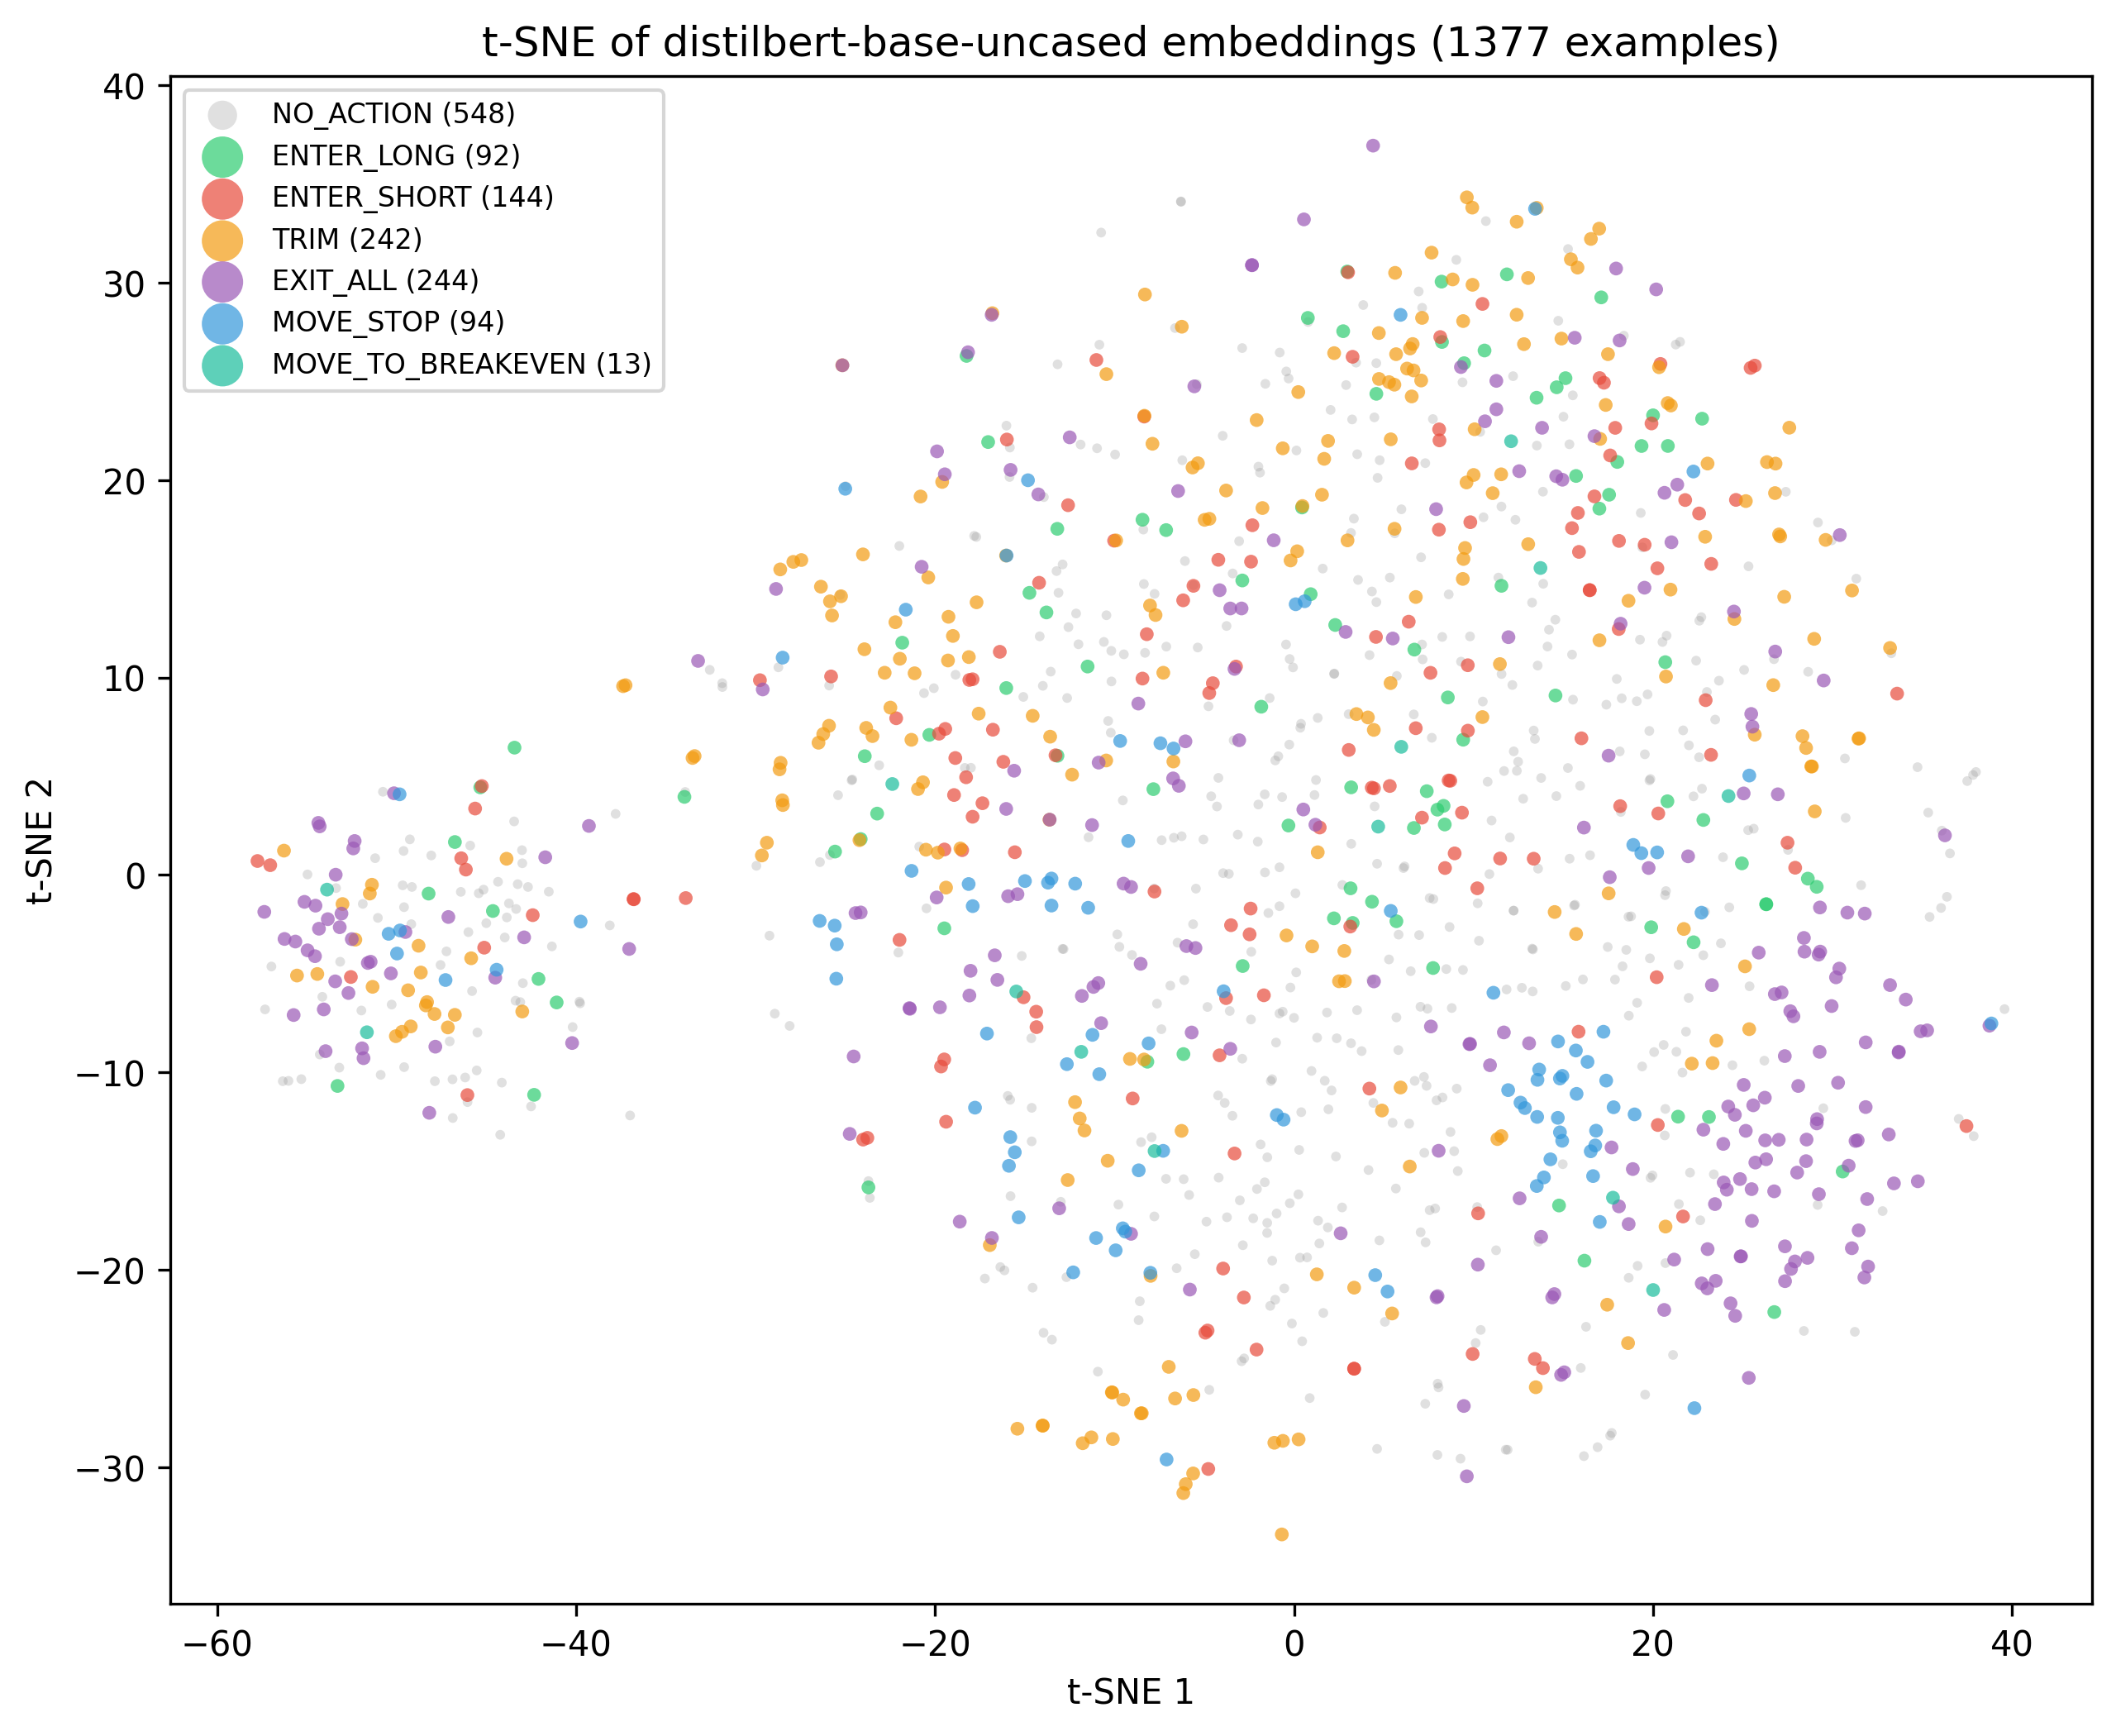
\includegraphics[width=0.49\textwidth]{tsne_distilbert.png}\hfill
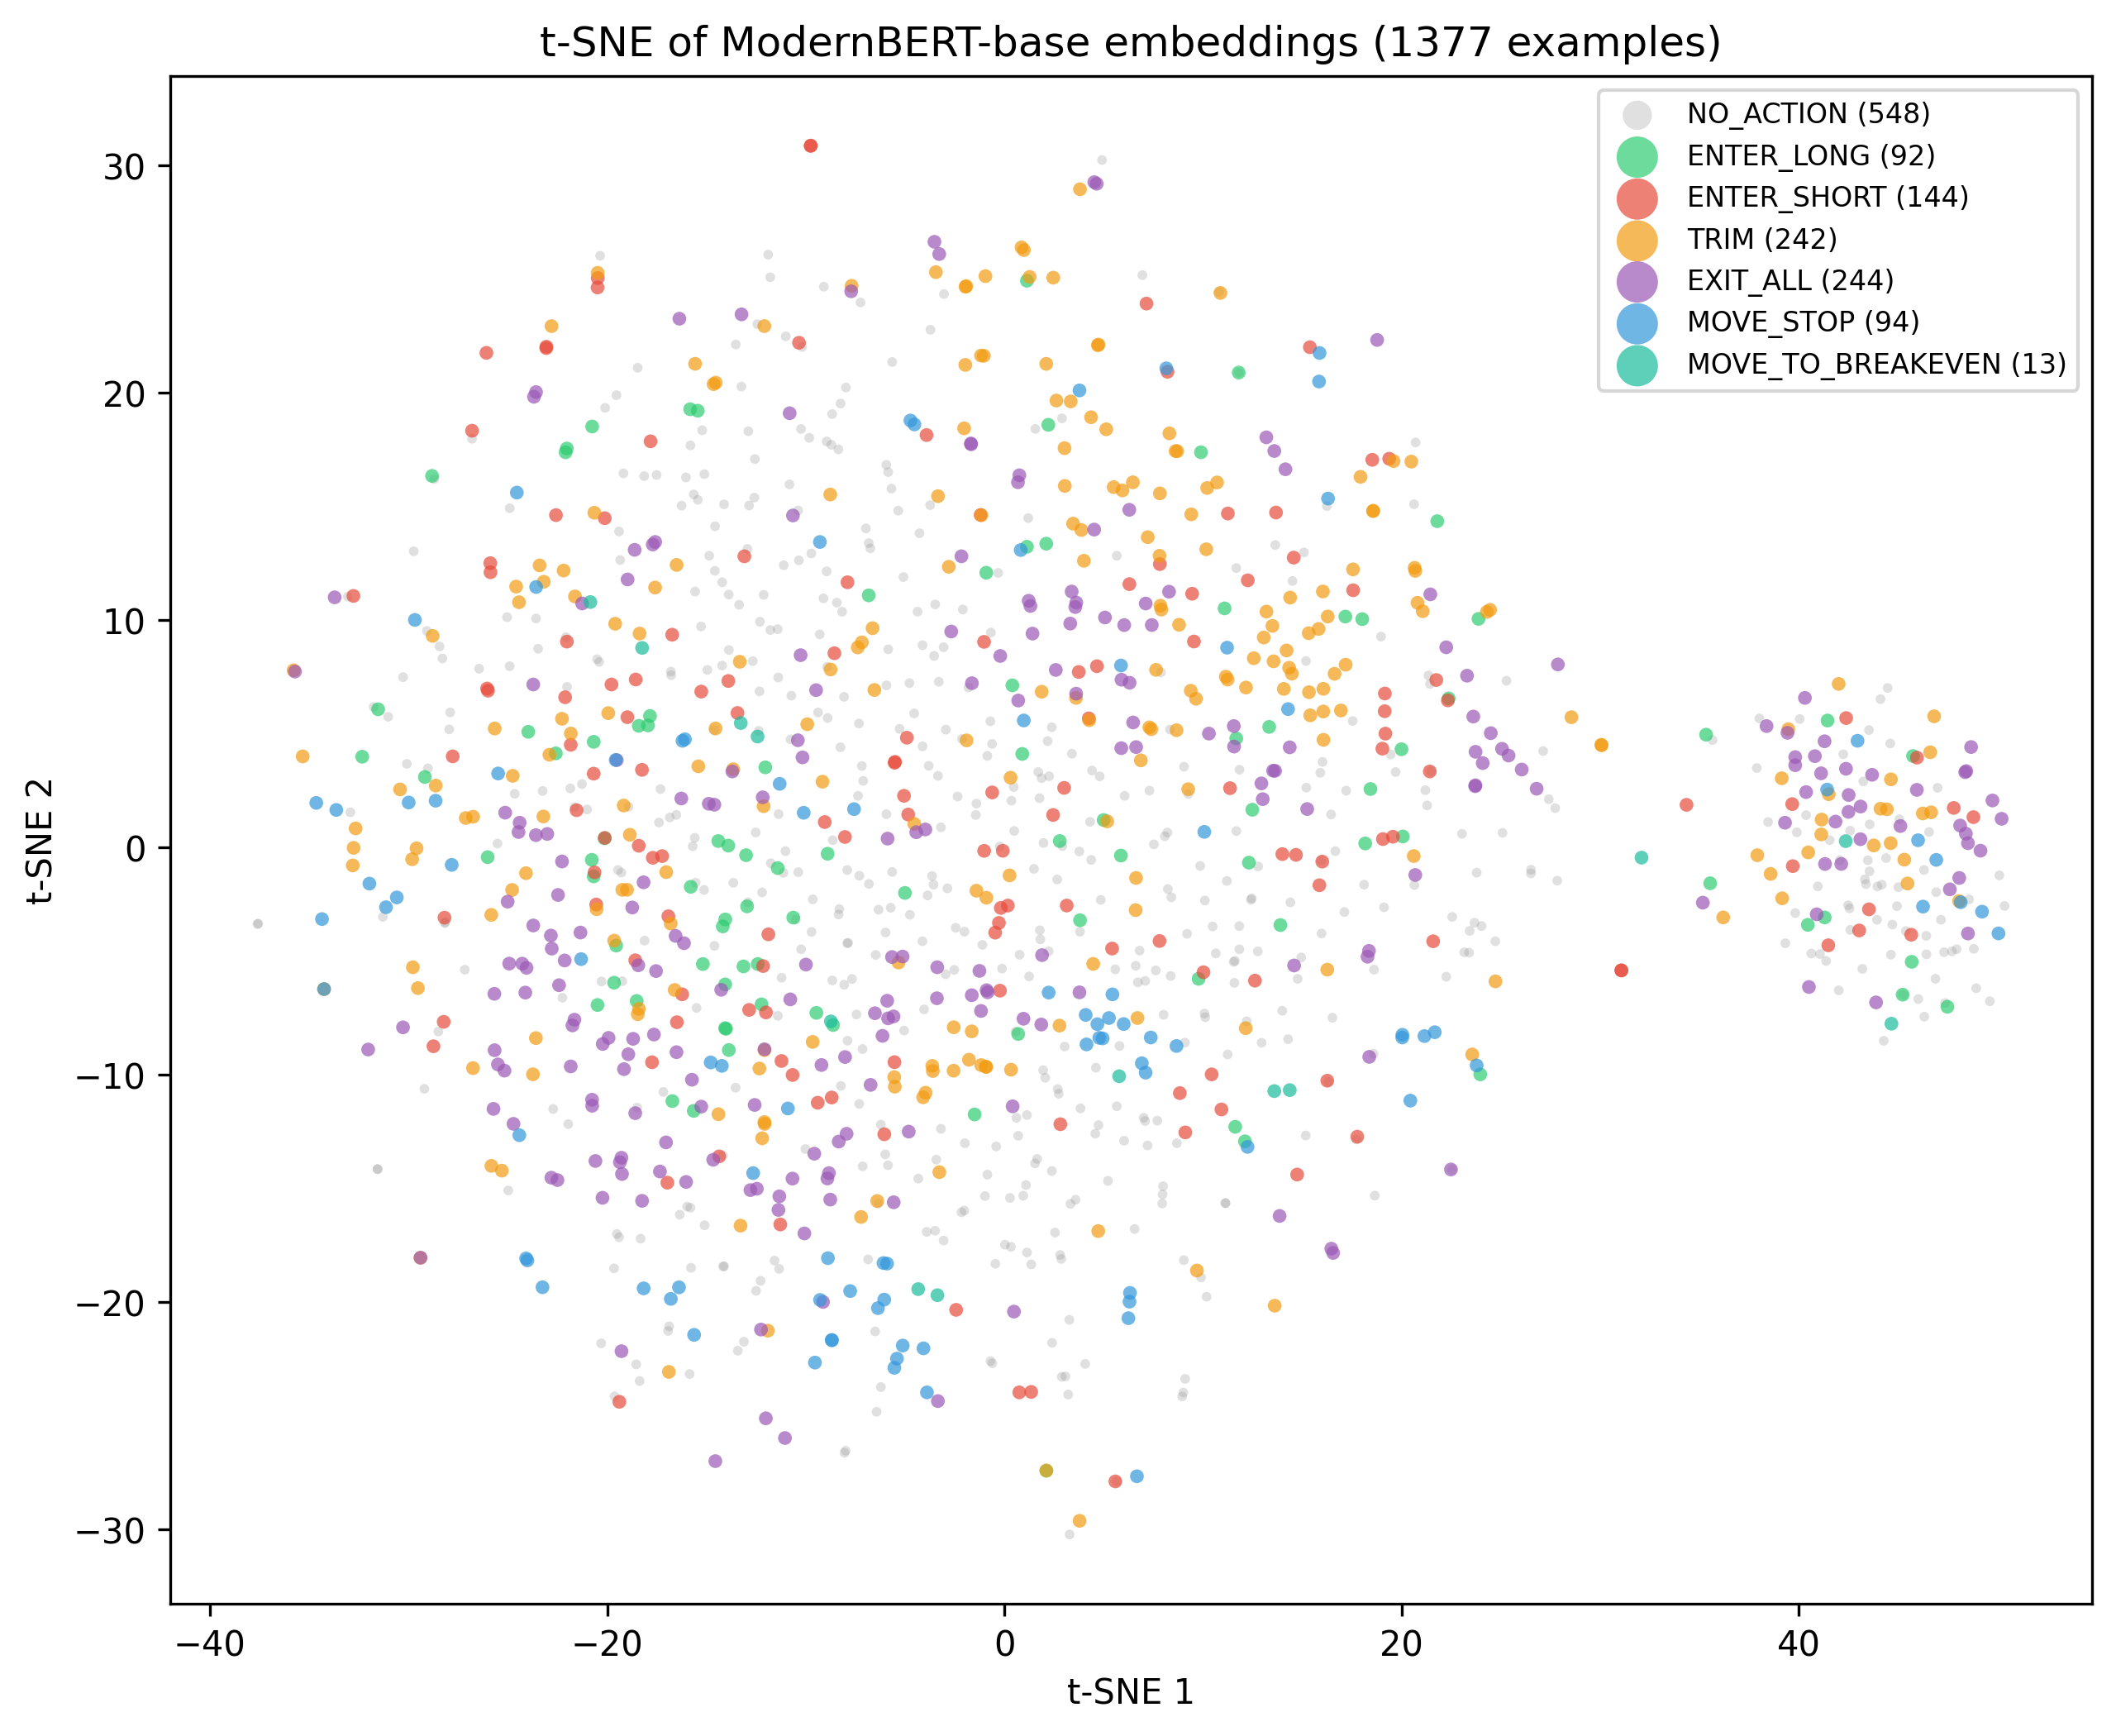
\includegraphics[width=0.49\textwidth]{tsne_modernbert.png}
\caption{t-SNE projections of frozen DistilBERT (left) and ModernBERT (right) embeddings for all 1.377 cleaned examples, coloured by true label.}
\label{fig:tsne}
\end{figure}

Both plots show no clear label-level clustering. All seven classes are heavily intermixed: \texttt{NO\_ACTION} spreads across the whole projected space, and the action classes overlap strongly with one another and with \texttt{NO\_ACTION}. DistilBERT retains slightly more loose sub-structure, but those groupings contain mixed labels and likely reflect transcript-level or syntactic similarity rather than trading intent, while ModernBERT's cloud is even more uniform. In both, \texttt{MOVE\_STOP} is the most spatially coherent class, consistent with the near-ubiquity of the word ``stop'' in its examples. t-SNE is a visualization, not a formal test, so this evidence is illustrative; but it fits the picture from the feature-importance analysis. ``Peeling some off'' (\texttt{TRIM}) and ``watching for longs'' (\texttt{NO\_ACTION}) can be close neighbours in general English, yet they need different labels; TF-IDF keeps them apart as distinct sparse features, whereas the frozen embeddings may place them side by side.

\subsection{Error Analysis}
\label{sec:error_analysis}

To characterize the practical failure modes of the best-performing model, all misclassifications from logistic regression's five-fold cross-validation on the cleaned dataset were collected: 299~errors out of 1.377~examples (21,7\%). Importantly, every one of these errors comes from the test side of a fold: each example was classified by a model that had never seen its transcript during training, so these are genuine generalization errors, not mistakes measured on training data. One caveat from the label check (Section~\ref{sec:label_verification}) carries over: the labelled actions are reliable, but not every real action carries a label. A prediction counted as a false positive against \texttt{NO\_ACTION} can therefore occasionally be a hit on one of those unlabelled actions rather than a genuine mistake. Table~\ref{tab:error_patterns} lists the ten most frequent error patterns.

\begin{table}[H]
\centering
\caption{Top 10 misclassification patterns for logistic regression on the cleaned dataset.}
\label{tab:error_patterns}
\begin{tabular}{@{}llcc@{}}
\toprule
\textbf{True Label} & \textbf{Predicted} & \textbf{Count} & \textbf{\% of Errors} \\
\midrule
\texttt{ENTER\_SHORT}  & \texttt{NO\_ACTION}   & 33 & 11,0 \\
\texttt{NO\_ACTION}    & \texttt{EXIT\_ALL}    & 32 & 10,7 \\
\texttt{NO\_ACTION}    & \texttt{ENTER\_SHORT} & 31 & 10,4 \\
\texttt{NO\_ACTION}    & \texttt{TRIM}         & 26 &  8,7 \\
\texttt{NO\_ACTION}    & \texttt{ENTER\_LONG}  & 25 &  8,4 \\
\texttt{ENTER\_SHORT}  & \texttt{ENTER\_LONG}  & 15 &  5,0 \\
\texttt{TRIM}          & \texttt{NO\_ACTION}   & 15 &  5,0 \\
\texttt{ENTER\_LONG}   & \texttt{ENTER\_SHORT} & 14 &  4,7 \\
\texttt{EXIT\_ALL}     & \texttt{TRIM}         & 12 &  4,0 \\
\texttt{TRIM}          & \texttt{EXIT\_ALL}    & 12 &  4,0 \\
\bottomrule
\end{tabular}
\end{table}

Examination of the misclassified examples reveals three dominant failure modes.

\textbf{Indirect entry language.} The most common error type (33 cases of \texttt{ENTER\_SHORT} $\rightarrow$ \texttt{NO\_ACTION}) arises when traders describe entries using past-tense, implicit, or unusual phrasing. For example, ``I did enter short versus New York here'' uses past tense; ``I've re-entered versus flow zones now'' uses an uncommon verb form; and ``All right. In it scalp here'' lacks an explicit directional keyword. The classifier has learned to trigger on standard patterns like ``short here'' or ``small short,'' and misses these variations.

\textbf{Exit-adjacent commentary.} The second pattern (32 cases of \texttt{NO\_ACTION} $\rightarrow$ \texttt{EXIT\_ALL}) occurs when the model over-triggers on exit-related language in non-action segments. Typical examples include ``Stopped me out by a point or two'' (describing a past stop-out, not a live action), ``Any push through 11s here. I'm out'' (a conditional statement), and ``There we build out this right shoulder'' (technical analysis where ``out'' appears in a non-exit context). The strong weight of the keyword ``out'' (+5,61) makes the model sensitive to any occurrence, including non-action uses.

\textbf{Advisory framing.} The third pattern (26 cases of \texttt{NO\_ACTION} $\rightarrow$ \texttt{TRIM}) involves second-person advice to viewers that superficially resembles self-directed action: ``Must be taking partials here, folks,'' ``Cover a little bit here into 600 just in case,'' and ``You can cover a piece here.'' The keywords ``partials,'' ``cover,'' and ``piece'' are strong \texttt{TRIM} signals, but the second-person framing (``you can,'' ``folks'') indicates advice rather than a trade the speaker is executing. The current text normalization pipeline does not distinguish between first-person and second-person constructions.

The error patterns point to concrete improvements: the model needs to pay more attention to verb tense (did something already happen, or is it happening now?), to who is being addressed (is the trader acting, or telling viewers what to do?), and to the difference between a plan and an executed action.

\subsection{How Large Does the Vocabulary Need to Be?}
\label{sec:vocab_ablation}

Here, vocabulary means the list of distinct words and word pairs that the TF-IDF step turns into features; its size was capped at 20.000 in all experiments. A final check verifies that this cap is neither a hidden bottleneck nor an inflated setting. The method is an \emph{ablation}: the same experiment is re-run several times with only one setting changed, here the maximum number of features. Logistic regression was evaluated with five-fold cross-validation on the cleaned dataset at caps of 5.000, 10.000, 20.000, and 50.000 features, yielding macro F1 of 0,700, 0,703, 0,703, and 0,703 respectively (accuracy 0,781/0,785/0,785/0,785; action F1 0,885/0,887/0,887/0,887). Performance saturates at 10.000 features, and raising the cap beyond that changes nothing, simply because the corpus only contains about 10.000 distinct unigrams and bigrams in the first place. Even 5.000 features capture 99,7\% of the top performance. The classification signal is concentrated in a compact set of domain-specific terms, and the 20.000-feature default is more than sufficient.

\subsection{From the Benchmark to Complete Sessions}
\label{sec:fullstream}

All results so far come from the AI-labelled dataset, in which trade actions are heavily overrepresented (Section~\ref{sec:label_verification}). The final experiments therefore ask the question that actually matters for deployment: what does the best model do when it has to read a real session from start to finish? Five complete livestream sessions were replayed line by line, 18.709 transcript lines covering 15,1 hours of streaming, and none of these lines were used for training anywhere in this thesis. Logistic regression was trained once on the cleaned dataset minus these five sessions and then asked to classify every single line, with prompts built by the same machinery that produced the training data.

The replay answers two questions. First, does the model still find the actions it should find? Largely yes: of the 23 labelled actions in these sessions, 18 (78\%) received an action prediction, 15 of them with exactly the right label, broadly in line with the action recall measured on the benchmark.

Second, and decisively: what else does it fire on? Here the picture collapses. Across the unlabelled lines, the model predicted an action 3.395 times, about 225 times per hour, while a day trader performs perhaps five to ten real actions per hour. The benchmark could not reveal this, because of a base-rate problem: when the thing being searched for is rare, even a decent detector produces mostly false alarms, just as a reliable medical screening test still produces mostly false positives when the disease itself is rare. In the benchmark, roughly every third line was an action; in a real session, fewer than one line in a hundred contains one.

How many of the 3.395 fires were actually right? To estimate this, a random sample of 100 fires (20 per session) was reviewed against the surrounding transcript. The review worked the same way the dataset itself was built: an AI model (Claude) read several lines of context around every fire and judged it, and the author then checked and confirmed the verdicts; every verdict is recorded with its reason in the evaluation files. The result: 3 of the 100 sampled fires were real trade actions that the dataset had simply never labelled, 5 were borderline, and 92 were clear false alarms. The model's standalone precision on a full stream is therefore roughly 3\%, and at most 8\% if every borderline case is counted in its favour, against 0,863 on the benchmark. The false alarms read like the error analysis of Section~\ref{sec:error_analysis} at scale: market analysis that contains trade words, reviews of past trades, conditional plans, and advice to viewers.

Could a stricter decision threshold fix this? No. Only 3 of the 3.395 false fires exceed the production system's confidence gate of 0,74, which sounds promising until one checks the other side: only 1 of the 18 correctly detected actions exceeds that gate as well. The model is unsure about everything, false alarms and real actions alike, so any threshold strict enough to silence the noise also silences the signal. Run on its own, the classifier is unusable on a real stream. How the production system avoids this fate is measured next.

Two design notes are needed for honesty. The position state during the replay was rebuilt from the 23 labelled actions, and since those are sparse, the state says ``no open position'' most of the time; this mirrors how the training prompts were built, but it pushes the model's mistakes towards entry predictions, which expect no open position. And the replay itself was checked for fidelity by comparing the prompts it rebuilds against the stored training prompts of these sessions: most match character for character, so the model really saw its familiar input format.

\subsection{The Full Pipeline on the Same Sessions}
\label{sec:fullstream_pipeline}

The numbers above describe the classifier running alone, which is not how the production system uses it. In production, the primary decision is made by the rule engine, the layer of several hundred hand-written text patterns introduced in Section~\ref{sec:pipeline}, and the classifier only assists: its confidence scores are used to veto doubtful rule matches and to recover actions the rules missed. As a closing comparison, the same five sessions were replayed through this real interpretation pipeline in three configurations: the rule engine alone, the rule engine with the deployed ModernBERT classifier, and the rule engine with the benchmark winner, TF-IDF logistic regression, in the classifier slot. During the replay, the position state evolved from the pipeline's own decisions, as it would in live trading, and a fired intent counts as detecting a labelled action when it lands within two lines of the labelled line. Table~\ref{tab:pipeline_fullstream} shows the outcome next to the standalone result.

\begin{table}[H]
\centering
\caption{The production interpretation pipeline on the five held-out sessions (15,1 hours), compared with the standalone classifier of Section~\ref{sec:fullstream}. Fires are action intents on lines that carry no action label.}
\label{tab:pipeline_fullstream}
\footnotesize
\setlength{\tabcolsep}{4pt}
\begin{tabular}{@{}lccc@{}}
\toprule
\textbf{Configuration} & \shortstack{\textbf{Labelled actions}\\\textbf{detected}} & \shortstack{\textbf{Exact}\\\textbf{label}} & \shortstack{\textbf{Fires}\\\textbf{per hour}} \\
\midrule
Standalone classifier (Section~\ref{sec:fullstream}) & 18 / 23 & 15 & $\sim$225 \\
Rule engine alone                                    &  5 / 23 &  5 & 5,4 \\
Rule engine + ModernBERT (production)                &  7 / 23 &  7 & 6,2 \\
Rule engine + TF-IDF logistic regr.                  &  7 / 23 &  7 & 6,3 \\
\bottomrule
\end{tabular}
\end{table}

Three things stand out.

First, the pipeline operates in an entirely different regime: roughly six fires per hour instead of 225, a thirty-five-fold reduction. And these fires are no longer mostly noise. Every fire of all three configurations (99 distinct transcript lines) was reviewed against the surrounding transcript, with the same AI-plus-author review process as the standalone sample. Of the 93 fires of the production configuration, 15 turned out to be real trade actions that simply carry no label in the dataset (live announcements such as ``I'm out of this now'' or ``stops into break even''), 8 were borderline, mostly the trader reporting an action he had executed moments earlier, and 70 were false alarms. So about one fire in six hits a real action, against roughly one in thirty for the standalone model, and the false alarms drop from around 210 per hour to about 4,6 per hour.

Second, the caution has a price. The pipeline detects only 7 of the 23 labelled actions, far below the standalone model's 18, because the rule engine refuses exactly the subtle phrasings (``Okay. Out. Oh, let it squeeze out.'') that the statistical model catches. What it does catch, it labels exactly right, every time. The system is built to prefer missing a trade over inventing one, and the numbers show that choice plainly.

Third, the classifier earns its supporting role, but which model fills that role makes almost no difference. Adding either classifier lifts detection from 5 to 7 of 23, at the cost of about one additional fire per hour, and the deployed ModernBERT and the benchmark-winning TF-IDF model produce nearly identical system behaviour, down to the share of real actions among their fires. Once the rules make the primary decision, the performance gap between the model families almost disappears.

What does this mean for practical use? As a fully automatic trade copier, the pipeline is not good enough yet: it would still trigger around four to five unjustified trades per hour while missing two thirds of the labelled actions. As an alerting assistant, where a human sees each proposed trade and confirms or rejects it, the numbers are workable: the alert rate is low enough to follow live, about every sixth alert points at a genuine action the dataset never knew about, and the detections it does make are labelled exactly right. The honest verdict is that the layered design turns an unusable classifier into a usable assistant, but not into an autonomous system.


% ═══════════════════════════════════════════════════════════════
% 5. DISCUSSION
% ═══════════════════════════════════════════════════════════════
\section{Discussion}
\label{sec:discussion}

\subsection{Why the Classical Models Win Here}
\label{sec:discussion_classical}

The most prominent finding of this work is that the TF-IDF-based linear models outperform the frozen transformer-head models on the aggregate metrics. Given how thoroughly transformers dominate recent NLP benchmarks, this deserves a short explanation, and the evidence for it has already appeared along the way.

Three strands of the explanation reinforce each other. The TF-IDF features are learned entirely from the training data, so they capture the domain's vocabulary automatically, while the frozen encoders, trained on general-purpose text, never had a reason to tell trading phrases such as ``peeling some off'' (a \texttt{TRIM}) and ``taking this off'' (\texttt{TRIM} or \texttt{EXIT\_ALL}, depending on context) apart. Trading language is also unusually repetitive: a small repertoire of fixed phrases announces most actions, and bigram features give each of these phrases its own dedicated dimension, which is exactly the sparse keyword signal the feature-importance analysis surfaced. And the comparison is asymmetric by design: the classical models adapt every parameter to the task, while the transformers may only train their tiny heads, so the part of them that can actually specialize in trading language is roughly ten times smaller than a linear TF-IDF model. The t-SNE plots close the loop: the frozen embeddings leave the seven classes intermixed, and a thin trained head cannot fix a space that never separated the classes in the first place. The result is consistent with the broader literature, where simple baselines remain competitive with deep learning on small or domain-specific text classification tasks~\cite{kowsari2019text}.

An important caveat applies. This study evaluates transformers exclusively in the feature-extraction setting (frozen encoder, trained head). The results show that \emph{frozen pretrained embeddings} do not beat TF-IDF on this task; they do not show that transformers in general are inferior. A fully fine-tuned transformer, or one adapted with parameter-efficient methods such as LoRA, might close or reverse the gap. The comparison here is between fully task-adapted classical models and minimally task-adapted transformers, which is not a level playing field for the transformers; it is, however, the realistic comparison when the dataset is too small to fine-tune safely.

\subsection{The Precision-Recall Tradeoff}
\label{sec:discussion_tradeoff}

The five models spread out along a clear precision-recall spectrum for action detection. The SVM and the balanced MLP favour precision (0,900 and 0,898 action precision), while ModernBERT favours recall (0,917 action recall). Logistic regression occupies the most balanced position, with action precision 0,863 and action recall 0,914, giving it the strongest action F1.

This tradeoff has direct practical implications, because the two error types cost different things. A false positive means executing a trade the trader never made; a false negative means missing a trade he did make. A deployment that prioritizes safety would favour a precision-leaning model such as the SVM, accepting that some signals are missed. A deployment that prioritizes completeness would favour high recall (the transformers), accepting more false alarms, which then must be caught by downstream safeguards. The balanced profile of logistic regression makes it the most versatile default.

\subsection{Which Actions Are Hard, and Why}
\label{sec:discussion_hierarchy}

The per-label results tell one consistent story across all five models. Management actions (\texttt{MOVE\_STOP}, \texttt{EXIT\_ALL}, \texttt{TRIM}) are the easiest, with F1 around 0,70--0,85, because traders announce them with explicit, almost ritual words: ``stop,'' ``out,'' ``partial.'' The \texttt{NO\_ACTION} class sits in the middle (F1 roughly 0,72--0,83), and varies across models because the boundary between no action and a subtly phrased action is genuinely blurry, all the more so given the incomplete action coverage of the labels. Entries (\texttt{ENTER\_LONG}, \texttt{ENTER\_SHORT}) are consistently hard (F1 roughly 0,48--0,64): entry language is varied and often implicit, and the model must also catch the direction, which may hide in an earlier sentence. \texttt{MOVE\_TO\_BREAKEVEN}, finally, remains the unstable outlier for the reason established earlier: there is simply almost no data for it.

This hierarchy suggests where improvement is cheapest. Entry classification would benefit most from additional training examples with diverse phrasing. For \texttt{MOVE\_TO\_BREAKEVEN}, the most pragmatic fix is structural rather than statistical: it could be merged into the closely related \texttt{MOVE\_STOP} class, since moving a stop to breakeven is a special case of moving a stop.

\subsection{Implications for Production Deployment}
\label{sec:discussion_production}

The benchmark winner is logistic regression, yet the production system runs ModernBERT in the classifier slot, a choice made before this benchmark existed. Should production simply switch to the best model? Looked at in isolation, yes: logistic regression classifies somewhat more accurately at no extra cost. But the full-stream experiments showed that the question matters less than it seems. No standalone classifier of either family could carry the live system, because on realistic input the false alarms vastly outnumber the real signals and no confidence threshold separates them. The architecture that follows is not a preference but a necessity: the rule engine, which fires rarely and precisely, makes the primary decision, and the classifier seconds it, vetoing doubtful rule matches and recovering clear misses. In that supporting role, the pipeline replay showed both models producing nearly identical system behaviour, so swapping the deployed model would change little. The deciding factors become practical ones instead, such as memory use and how easy the trained model is to ship, and an end-to-end evaluation including live execution would still be needed before swapping any component. The real lever for improving the system is not the choice between these two classifiers but the training data itself (Section~\ref{sec:future_work}).

Latency deserves its own mention, because in trading it matters nearly as much as accuracy: a signal that arrives seconds late gets executed at a worse price, and the production risk engine deliberately discards signals that are too old. Within the pipeline, by far the slowest part is getting from speech to final text. The system first has to wait for the trader to finish the utterance (segments run up to about four seconds), transcription itself adds a few hundred milliseconds, and the transcription queue is kept deliberately short so that a fast talker cannot build up a backlog of stale audio. Classification, in contrast, takes only milliseconds to a few tens of milliseconds, for the classical models and the transformer head alike. Model choice therefore barely moves the end-to-end latency; speech-to-text dominates it, and any future latency work should start there.

\subsection{Ethical, Legal, and Operational Risk}
\label{sec:ethics_risk}

The application context raises risks that are separate from classification accuracy. A false positive in a trade-copying system is not merely a labelling error; if connected to execution infrastructure, it could create an unintended market order. Any production deployment should therefore keep human override controls, confidence thresholds, stale-signal checks, position-size limits, and audit logs in place. The evaluation in this thesis measures text classification only and should not be interpreted as evidence that fully automated execution is safe.

The data source also requires care. Livestream transcripts are public-facing media, but automated collection and reuse may still be constrained by platform terms, copyright, or streamer-specific expectations. This thesis uses archived transcripts for research; an operational system should verify that its collection, storage, and use of transcript data are permitted. Finally, detected trade signals should not be presented as financial advice. The system classifies what a speaker appears to say; it does not evaluate whether the trade is suitable, lawful, or economically sound.

\subsection{Limitations}
\label{sec:limitations}

Several limitations of this work should be acknowledged.

\textbf{Benchmark composition, and the scope of the full-stream test.} The primary results (Sections~\ref{sec:results_cleaned} to~\ref{sec:vocab_ablation}) were measured on the curated benchmark corpus, in which trade actions are heavily overrepresented, and must not be read as deployment accuracy. The full-stream evaluation (Section~\ref{sec:fullstream}) was added precisely to measure that gap, and it found a severe one: standalone precision of only a few percent on complete sessions. That test has limits of its own, however. It covers five sessions with only 23 labelled actions, so its recall estimate is coarse; the position state during the replay was reconstructed from the sparse labels and was therefore flat most of the time; and the precision estimate rests on a 100-fire sample, reviewed by an AI model and confirmed by the author, rather than on a fully labelled stream. The pipeline replay (Section~\ref{sec:fullstream_pipeline}) shares these limits, although its fires were at least all individually reviewed with the same AI-plus-author process. The benchmark results remain what they were designed to be, a controlled comparison between model families; the full-stream results give the direction and rough size of the deployment gap, not a precise production error rate.

\textbf{Dataset size.} At 1.442 cleaned examples (1.377 after deduplication) across 103 transcripts, the dataset is small. The results may not generalize to larger or differently distributed datasets, and the relative ranking of classical versus transformer models could change with substantially more training data, particularly if full fine-tuning becomes feasible.

\textbf{Single domain.} All transcripts come from a single trader and a single instrument (Nasdaq futures). Different traders, instruments, or trading styles may use different language that requires separate training.

\textbf{Frozen encoders.} The transformer models were evaluated exclusively with frozen encoder weights. Full fine-tuning, parameter-efficient fine-tuning (such as LoRA), or continued pretraining on trading-domain text might substantially improve their performance but were not explored.

\textbf{Imperfect labels.} The labels were generated by LLMs and reviewed by the author, and the manual verification (Section~\ref{sec:label_verification}) found them precise but incomplete: not every action in the streams is labelled, and some \texttt{NO\_ACTION} lines may contain weak or repeated actions. The labels also record only what the trader announced; without broker statements there is no proof that an announced trade was actually placed. Finally, the labelled lines were not sampled at random. Lines with clear trade wording were more likely to be selected for labelling in the first place, and two accepted labels were ambiguous even to a human reader. This selection makes the classes look cleaner than the underlying speech is, and it can make the measured error rates, especially the false-positive rate, look better than they would on unselected speech.

\textbf{Each line judged in isolation.} The classifier treats every transcript segment independently, although trading actions occur in sequences (entry, then management, then exit). A model aware of this temporal structure could rule out impossible predictions and resolve ambiguous lines from their context.

\subsection{Future Work}
\label{sec:future_work}

Several directions follow from the findings and limitations.

\textbf{Training with realistic class balance.} The training data presents the model with one action for every 2,5 non-actions, while a real stream contains over a hundred non-action lines per action. The full-stream test (Section~\ref{sec:fullstream}) showed where that mismatch leads. Retraining with far more hard negative examples, precisely the analysis-with-trade-words chatter that causes the false alarms, is the most direct way to close the measured precision gap.

\textbf{Fully labelled full-stream evaluation.} The full-stream test relied on the 23 labelled actions of five sessions and a sampled review of the model's fires. Labelling several entire sessions exhaustively, every line, would turn the sampled precision estimate into an exact one, allow recall to be measured beyond the existing labels, and give the position-state replay a complete action sequence to work with.

\textbf{Full fine-tuning with more data.} Expanding the labelled set to several thousand examples across multiple traders and then fine-tuning the entire encoder, instead of keeping it frozen, is the most direct path to stronger transformer performance; at 5.000--10.000 examples, overfitting becomes manageable with standard regularization.

\textbf{Parameter-efficient fine-tuning.} Methods such as LoRA adapt a pretrained model by training only a small number of additional parameters, a middle ground between frozen feature extraction and full fine-tuning that could be feasible even at the current dataset size.

\textbf{Sequence-aware modelling.} The classifier currently judges every segment on its own, even though trades unfold in order: an exit can only follow an entry, and a stop can only be moved while a position is open. A model that reads consecutive segments together, or that carries the running position state from one prediction into the next, could rule out impossible actions and recover entries that only become clear over two or three lines.

\textbf{Domain-specific pretraining.} Continued pretraining on a large corpus of unlabelled trading transcripts, which are freely available on YouTube, could adapt the embeddings to trading vocabulary and reduce the mismatch with general-purpose pretraining data.

\textbf{End-to-end evaluation with execution.} Section~\ref{sec:fullstream_pipeline} replayed the interpretation pipeline offline. An end-to-end test that adds the optional LLM confirmation layer, live transcription noise, and the risk and execution stages, ideally judged against broker records, remains open.


% ═══════════════════════════════════════════════════════════════
% 6. SUMMARY
% ═══════════════════════════════════════════════════════════════
\section{Summary}
\label{sec:summary}

This work addressed the question of which machine learning approach provides the most accurate trade-intent classification from noisy livestream transcripts, comparing classical TF-IDF-based methods with frozen transformer feature extractors.

\textbf{Question.} Given a short transcript segment from a daytrading livestream and the current trading context, which model family best predicts the trader's intended action from a set of seven classes (no action, enter long, enter short, trim, exit all, move stop, move to breakeven)? Which action classes are most and least amenable to automated detection, and what systematic error patterns emerge?

\textbf{Procedure.} From 103 transcribed YouTube livestreams, 1.466 lines were labelled with the help of three large language models and reviewed by hand; cleanup and deduplication leave 1.377 unique examples for the primary evaluation. A manual check of 203 action labels confirmed nearly all of them, but also showed that not every action in the streams is labelled, so the benchmark is action-enriched rather than a complete record. Five models were compared under identical conditions: logistic regression, a linear SVM, and an MLP on TF-IDF features, and DistilBERT and ModernBERT as frozen encoders with small trained classification heads. Evaluation used five-fold cross-validation, split by transcript so that no model is ever tested on a session it trained on. A closing experiment replayed five complete held-out sessions, more than 18.000 lines, through the best model.

\textbf{Results.} On the cleaned dataset, logistic regression achieved the best macro F1 (0,703) and action F1 (0,887), while the SVM achieved the best accuracy (0,795) and action precision (0,900). ModernBERT achieved the highest action recall (0,917) but lower precision and macro F1. The MLP improved markedly with balanced oversampling (macro F1 from 0,572 to 0,634) but still trailed both linear models. Data cleanup improved most metrics. The supporting analyses explain the gap: classification is driven by a small set of domain keywords that TF-IDF captures directly, the frozen embeddings show no label-level structure under t-SNE, and the dominant error modes are indirectly phrased entries, exit-like commentary, and advice to viewers mistaken for action. A vocabulary ablation showed performance saturating at about 10.000 features. The full-stream experiment then showed the second central finding of this work: the benchmark numbers do not transfer to complete sessions. Reading five full held-out sessions, the best model still found 18 of 23 labelled actions, but fired about 225 times per hour, of which only a few percent were real actions, so on its own it would be unusable live. The cause is the rarity of real actions in natural speech, and the consequence is the layered production design in which hand-written rules decide and the classifier merely assists. A replay of that full pipeline over the same sessions confirmed the design: it fires only about six times per hour, a review of every one of those fires showed that about one in six points at a real trade action the dataset never labelled, the classifier layer adds detections the rules miss, and the choice of assisting model, ModernBERT or TF-IDF, barely changes the system's behaviour (Sections~\ref{sec:fullstream} to~\ref{sec:discussion_production}).

These results show that for small, domain-specific text classification tasks with repetitive, keyword-driven language, classical machine learning methods on TF-IDF features remain highly competitive. The added complexity of pretrained transformer feature extraction does not translate into better performance when the encoder is frozen and the training set is small.

For practitioners facing similar tasks, classification on small, specialised, and often noisy corpora, the practical lesson is to start with simple, well-understood baselines before investing in heavier architectures, and to evaluate them under conditions as close as possible to deployment. The dominance of pretrained transformers on standard benchmarks does not automatically transfer to every setting; when the encoder cannot be fine-tuned and the classification signal concentrates in a small set of domain keywords, a TF-IDF model with a balanced linear classifier is a competitive, interpretable, and easy-to-deploy choice.

The source code of the system and of the complete benchmark pipeline is publicly available at \url{https://github.com/AndiCodesss/bachelor_thesis}. Apart from five example transcripts that show the data format, the recorded transcripts and the labelled dataset are not included in the repository, mainly because of their size, so the repository documents the pipeline and its stored results rather than providing a rerunnable copy of the experiments (Section~\ref{sec:reproducibility}).


% ═══════════════════════════════════════════════════════════════
% BIBLIOGRAPHY
% ═══════════════════════════════════════════════════════════════
\newpage



\bibliographystyle{plainnat}
\bibliography{MyReferences}

\end{document}
